% KINETIQ B.Tech Minor Project Report
% Build with: xelatex main && biber main && xelatex main && xelatex main
\documentclass[12pt,a4paper,oneside]{report}

\usepackage[a4paper,top=25mm,bottom=25mm,left=32mm,right=25mm]{geometry}
\usepackage{fontspec}
\setmainfont{TeX Gyre Termes}
\setsansfont{TeX Gyre Heros}
\usepackage{microtype}
\usepackage{setspace}
\onehalfspacing
\usepackage{graphicx}
\graphicspath{{figures/}}
\usepackage{booktabs,tabularx,longtable,array,multirow}
\usepackage{enumitem}
\usepackage{float}
\usepackage{caption,subcaption}
\usepackage[table]{xcolor}
\usepackage{tikz}
\usetikzlibrary{arrows.meta,positioning,shapes.geometric,fit,calc}
\usepackage{fancyhdr}
\usepackage{titlesec}
\usepackage{listings}
\usepackage{csquotes}
\usepackage[backend=biber,style=numeric,sorting=none,maxbibnames=99]{biblatex}
\addbibresource{references.bib}
% Allow line breaks inside bibliography URLs (avoids overfull bibliography lines)
\setcounter{biburlnumpenalty}{100}
\setcounter{biburlucpenalty}{100}
\setcounter{biburllcpenalty}{100}
\usepackage[colorlinks=true,linkcolor=black,citecolor=black,urlcolor=blue!60!black,pdfauthor={Sidharth Sajith and Tharun Oommen Jacob},pdftitle={KINETIQ -- Real-Time Wellness Mirror with FreeRTOS and Sensor-Grounded AI}]{hyperref}

\definecolor{kinetiqBlue}{HTML}{173B61}
\definecolor{kinetiqTeal}{HTML}{147D7E}
\definecolor{kinetiqGreen}{HTML}{3B7A57}
\definecolor{kinetiqOrange}{HTML}{B96A1B}
\definecolor{softBlue}{HTML}{EAF2F8}
\definecolor{softGreen}{HTML}{EAF5EC}
\definecolor{softOrange}{HTML}{FFF3E4}
\definecolor{softGray}{HTML}{F3F5F6}

\captionsetup{font=small,labelfont=bf,justification=centering}
\setlist[itemize]{leftmargin=7mm,noitemsep,topsep=2pt}
\setlist[enumerate]{leftmargin=8mm,noitemsep,topsep=2pt}
\renewcommand{\arraystretch}{1.22}
\newcolumntype{Y}{>{\raggedright\arraybackslash}X}
\newcolumntype{C}{>{\centering\arraybackslash}m{0.15\textwidth}}
\newcommand{\placeholder}[1]{\textit{[#1]}}
\newcommand{\code}[1]{\texttt{#1}}
\newcommand{\tmark}{\textcolor{kinetiqGreen}{\textbf{Verified}}}
\newcommand{\pmark}{\textcolor{kinetiqOrange}{\textbf{Qualified}}}
\newcommand{\nmark}{\textcolor{red!65!black}{\textbf{Not demonstrated}}}

\titleformat{\chapter}[display]
  {\normalfont\bfseries\color{kinetiqBlue}}
  {\filleft\Large CHAPTER \thechapter}
  {1ex}{\titlerule\vspace{1.2ex}\filright\Huge}
\titlespacing*{\chapter}{0pt}{-10pt}{20pt}
\titleformat{\section}{\large\bfseries\color{kinetiqBlue}}{\thesection}{0.75em}{}
\titleformat{\subsection}{\normalsize\bfseries\color{kinetiqTeal}}{\thesubsection}{0.75em}{}

\pagestyle{fancy}
\fancyhf{}
\fancyhead[L]{\small KINETIQ}
\fancyhead[R]{\small Real-Time Wellness Mirror}
\fancyfoot[C]{\thepage}
\renewcommand{\headrulewidth}{0.3pt}
\setlength{\headheight}{15pt}
\fancypagestyle{plain}{\fancyhf{}\fancyfoot[C]{\thepage}\renewcommand{\headrulewidth}{0pt}}

\lstset{basicstyle=\ttfamily\footnotesize,frame=single,breaklines=true,backgroundcolor=\color{softGray},xleftmargin=2mm,xrightmargin=2mm}

\begin{document}
\pagenumbering{roman}
\begin{titlepage}
  \centering
  \vspace*{9mm}
  
\includegraphics[width=27mm]{ppt_image1.png}\par\vspace{8mm}
  {\Large\bfseries SAINTGITS COLLEGE OF ENGINEERING\par}
  {\large (Autonomous), Kottayam\par}
  \vspace{13mm}
  {\Large\bfseries B.TECH MINOR PROJECT REPORT\par}
  \vspace{11mm}
  {\large entitled\par}\vspace{5mm}
  {\LARGE\bfseries\color{kinetiqBlue} KINETIQ\par}
  \vspace{3mm}
  {\Large\bfseries Real-Time Wellness Mirror with FreeRTOS and Sensor-Grounded AI\par}
  \vspace{13mm}
  {\large Submitted by\par}\vspace{4mm}
  {\large\bfseries Sidharth Sajith \quad and \quad Tharun Oommen Jacob\par}
  \vspace{12mm}
  {\large Under the guidance of\par}\vspace{4mm}
  {\large\bfseries Er. Jittu George Eapen\par}
  {\large Assistant Professor\par}
  \vfill
  {\large\bfseries Department of Electronics Engineering\par}
  \vspace{4mm}
  {\large Saintgits College of Engineering (Autonomous), Kottayam\par}
  \vspace{7mm}
  {\large Academic year: \placeholder{to be entered by the department}\par}
\end{titlepage}

\clearpage
\thispagestyle{empty}
\begin{center}
{\Large\bfseries CERTIFICATE}\par\vspace{14mm}
\end{center}
\noindent This is to certify that the B.Tech Minor Project entitled \textbf{``KINETIQ -- Real-Time Wellness Mirror with FreeRTOS and Sensor-Grounded AI''} is a record of work carried out by \textbf{Sidharth Sajith} and \textbf{Tharun Oommen Jacob} in the Department of Electronics Engineering, Saintgits College of Engineering (Autonomous), Kottayam, under the guidance of \textbf{Er. Jittu George Eapen}, Assistant Professor. The institutional approvals, register numbers, submission date, and signatures shall be completed by the authorised office.
\vspace{28mm}
\begin{tabularx}{\textwidth}{>{\centering\arraybackslash}Y >{\centering\arraybackslash}Y}
\rule{55mm}{0.4pt}\par Supervisor\par Er. Jittu George Eapen &
\rule{55mm}{0.4pt}\par Head of Department\par \placeholder{Authorised signatory}\\[25mm]
\rule{55mm}{0.4pt}\par Project Coordinator\par \placeholder{Authorised signatory} &
\rule{55mm}{0.4pt}\par Principal\par \placeholder{Authorised signatory}\\
\end{tabularx}
\vfill
\noindent Place: Kottayam \hfill Date: \placeholder{to be entered}

\clearpage
\chapter*{ACKNOWLEDGEMENTS}
\addcontentsline{toc}{chapter}{Acknowledgements}
The authors record sincere gratitude to Er. Jittu George Eapen, Assistant Professor, for technical guidance and review. Appreciation is extended to the Department of Electronics Engineering and Saintgits College of Engineering (Autonomous) for the academic environment supporting the work. The documented implementation also benefited from the project team's test materials, device records, and software artefacts.

\clearpage
\chapter*{ABSTRACT}
\addcontentsline{toc}{chapter}{Abstract}
KINETIQ is a local wellness-mirror prototype that combines two deliberately distinct telemetry pathways with a common validation and assistance layer. The genuine-data pathway transports observations from a Huawei Band 6 through Huawei Health and an Android accessibility streaming service to an authenticated local receiver. The receiver and bridge admit only complete, fresh, non-simulated values before forwarding a constrained mirror payload. A separate native FreeRTOS v11 application demonstrates deterministic activity-control behaviour with synthetic telemetry, queue and timing diagnostics, and an operator-controlled fallback. Both pathways terminate at a laptop-based mirror that exposes source, link, freshness, and data-quality state instead of presenting cached values as live.

The shared contract contains eight fields: timestamp, heart rate, oxygen saturation, activity, motion intensity, exertion, steps, and PPG quality. Schema, range, completeness, source, and freshness checks gate dashboard and assistant inputs. The assistant receives accepted context, returns a bounded wellness-oriented response, displays a grounding verdict, and retains an offline deterministic template when the optional local language-model service is unavailable. The implementation is explicitly non-clinical: it neither diagnoses nor treats a condition.

Repository evidence includes authenticated receiver records containing 60 BPM, 100\% SpO\textsubscript{2}, stress 57, and 4,181 steps on 22 October 2026; a separate synthetic dashboard session containing 75 frames over 15 seconds with no recorded drops; a 30-message BLE mock; and a 0.48 s faster-whisper result on synthesized audio. These observations establish bounded portions of the pipeline only. Physical ESP32 sensing remains represented by component selection and Wokwi simulation rather than a verified final hardware acquisition.

\noindent\textbf{Keywords:} FreeRTOS, wearable telemetry, data freshness, wellness mirror, schema validation, sensor-grounded AI, Huawei Health.

\clearpage
\tableofcontents
\clearpage
\listoffigures
\addcontentsline{toc}{chapter}{List of Figures}
\clearpage
\listoftables
\addcontentsline{toc}{chapter}{List of Tables}
\clearpage
\chapter*{ABBREVIATIONS}
\addcontentsline{toc}{chapter}{Abbreviations}
\begin{longtable}{p{38mm}p{105mm}}
\textbf{AI} & Artificial Intelligence \\
\textbf{BLE} & Bluetooth Low Energy \\
\textbf{BOM} & Bill of Materials \\
\textbf{CSV} & Comma-Separated Values \\
\textbf{ESP32} & Espressif 32-bit microcontroller family \\
\textbf{HWM} & High-Water Mark \\
\textbf{IMU} & Inertial Measurement Unit \\
\textbf{JSON} & JavaScript Object Notation \\
\textbf{LLM} & Large Language Model \\
\textbf{PPG} & Photoplethysmography \\
\textbf{RTOS} & Real-Time Operating System \\
\textbf{SpO\textsubscript{2}} & Peripheral oxygen saturation \\
\textbf{STT} & Speech-to-Text \\
\textbf{TTS} & Text-to-Speech \\
\textbf{UI} & User Interface
\end{longtable}

\clearpage
\pagenumbering{arabic}
\setcounter{page}{1}
\chapter{INTRODUCTION}

\section{Background and Motivation}
Wearable devices can make physiological observations available continuously, but a value on a wearable application screen is not automatically a current, validated value at a second interface. Transport delay, incomplete packets, cached application screens, and loss of connectivity can all separate the observation from its later presentation. A wellness interface that obscures those conditions risks making stale values appear live. KINETIQ addresses that interface and integration problem with explicit provenance, freshness, and validation states.

The implementation joins a Huawei Band 6 and Huawei Health data path to a laptop-based wellness mirror through a local Android accessibility streaming service and authenticated receiver. Android accessibility services are intended to observe and assist interaction with user-interface content under a user-granted permission model \cite{androidAccessibility}. No direct Huawei Band application-programming-interface integration is claimed: the genuine pathway depends on data rendered by Huawei Health and captured by the phone-side service. The distinction matters because a visible Huawei Health value, a receiver record, an accepted bridge payload, and a rendered mirror value represent different stages of evidence.

KINETIQ also contains a separate native FreeRTOS v11 control pathway. Its virtual activity states and generated telemetry provide a deterministic, inspectable control demonstration when wearable transport is unavailable. FreeRTOS queues provide safe task-to-task data transfer, while mutexes protect a shared resource from concurrent access \cite{freertosQueues,freertosMutex}. The pathway is intentionally synthetic; its values are never presented as a person's physiological measurements.

\section{Engineering Problem}
Generic conversational assistance lacks direct access to the state that a user sees on a wellness dashboard. Conversely, passing arbitrary or stale telemetry to an assistant can make a fluent answer appear more reliable than its input. The engineering problem is therefore to combine local telemetry processing and wellness assistance while retaining five properties:

\begin{itemize}
  \item a traceable distinction between genuine wearable observations and synthetic control telemetry;
  \item rejection of malformed, incomplete, simulated, or non-live input before presentation;
  \item visible indication of transport link, source, and data freshness;
  \item deterministic fallback behaviour with observable task timing and queue condition; and
  \item bounded, context-conditioned wellness guidance without a diagnostic or treatment claim.
\end{itemize}

The problem is constrained by the available implementation. The current genuine pathway proves documented receiver-side records and bridge eligibility rules, not a universal end-to-end guarantee for every Huawei Health screen or measurement. Physical ESP32 sensor acquisition is similarly outside the verified final runtime. Hardware selection and Wokwi artefacts provide design and simulation evidence rather than a claim of deployed sensor readings.

\section{Limitations of Unqualified Wellness Interfaces}
An interface can be technically misleading even when every displayed number originated at a legitimate device. A heartbeat value may be historical rather than real-time; a route may drop a field; a receiver may accept a packet with an old timestamp; or a dashboard may retain its last good value after the sender disconnects. KINETIQ treats arrival time, value-change time, and freshness state as first-class UI data. After the configured offline threshold, the mirror blanks the measurement rather than retaining it in a live-looking card.

The same caution applies to AI output. Context-grounded response generation can constrain an assistant to the accepted snapshot, but a displayed grounding verdict does not establish medical accuracy, clinical safety, or suitability for a particular person. KINETIQ is a wellness-assistance prototype. It does not provide medical diagnosis, treatment, emergency detection, or clinical alerting.

\section{Objectives}
The implemented objectives are organised around evidence separation and controllable operation:

\begin{enumerate}
  \item implement an observable native FreeRTOS control lane with activity commands, task timing, queue diagnostics, and synthetic telemetry;
  \item ingest Huawei Health user-interface observations through a phone-side relay and authenticated local receiver without claiming a direct Huawei Band API;
  \item define and enforce a shared eight-field telemetry contract before dashboard or assistant consumption;
  \item make source, link, freshness, and quality state visible to the operator;
  \item generate context-conditioned wellness responses with a visible grounding \texttt{PASS}/\texttt{FAIL} verdict and offline fallback; and
  \item document repeatable demonstrations, test scope, and unverified hardware boundaries.
\end{enumerate}

\section{Scope and Boundaries}
The laptop application is local-only in the examined configuration: its HTTP receiver binds to the loopback interface. The phone relay sends authenticated POST requests to the local receiver. The bridge emits a strict mirror schema only when HR, SpO\textsubscript{2}, and steps are present, valid, non-simulated, and classified as live by the relay contract. Stress observations are retained in documented receiver records but are not among the eight shared mirror fields and are not forwarded by the examined bridge.

The control lane accepts keyboard commands \texttt{1} (Rest), \texttt{2} (Walk), \texttt{3} (Run), \texttt{b} (Fall event), and \texttt{0} (Automatic mode). It is a Windows-hosted FreeRTOS simulator and cannot establish hard real-time behaviour of a deployed microcontroller. The planned embedded scope identifies an ESP32 DevKit V1, MPU6050, HC-SR04, infrared sensing, DHT22, supporting components, and a Wokwi route. Those materials are retained as design evidence only.

\section{Dual-Pathway Overview}
Figure~\ref{fig:intro-dual} summarises the design principle. The genuine lane preserves provenance from the wearable application path. The deterministic lane supplies explicitly synthetic control telemetry. Both pass through a shared contract and dashboard surface, but their source labels remain separate. That separation prevents the control lane from becoming an unmarked substitute for a user measurement.

\begin{figure}[H]
\centering
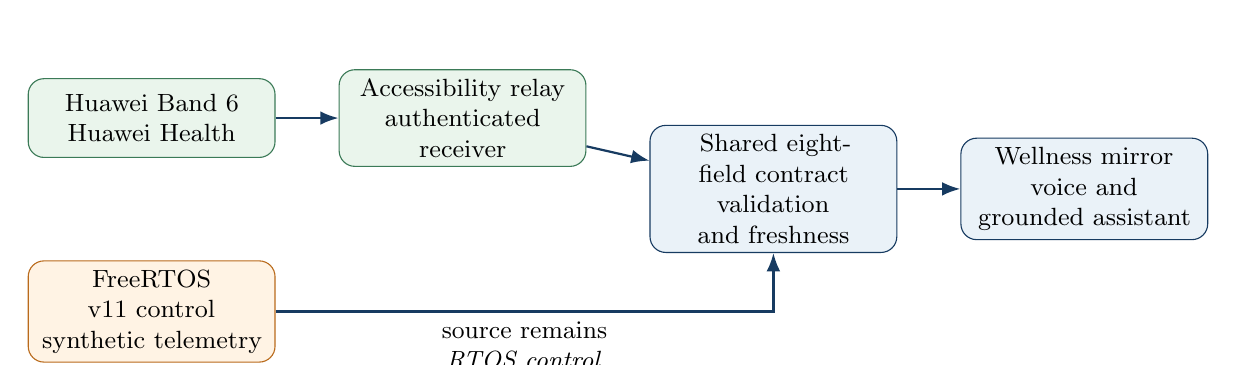
\begin{tikzpicture}[font=\small, node distance=7mm and 8mm, >=Latex,
 box/.style={draw=kinetiqBlue, rounded corners=2mm, align=center, minimum height=10mm, text width=29mm, fill=softBlue},
 greenbox/.style={box,draw=kinetiqGreen,fill=softGreen},
 orangebox/.style={box,draw=kinetiqOrange,fill=softOrange},
 flow/.style={->,thick,draw=kinetiqBlue}]
\node[greenbox] (wear) {Huawei Band 6\\Huawei Health};
\node[greenbox,right=of wear] (relay) {Accessibility relay\\authenticated receiver};
\node[orangebox,below=13mm of wear] (rtos) {FreeRTOS v11 control\\synthetic telemetry};
\node[box,right=of relay,yshift=-9mm] (gate) {Shared eight-field contract\\validation and freshness};
\node[box,right=of gate] (mirror) {Wellness mirror\\voice and grounded assistant};
\draw[flow] (wear)--(relay);
\draw[flow] (relay)--(gate);
\draw[flow] (rtos.east)-| node[pos=.25,below,align=center]{source remains\\\textit{RTOS control}} (gate.south);
\draw[flow] (gate)--(mirror);
\end{tikzpicture}
\caption[Two telemetry pathways with a shared mirror interface]{KINETIQ uses two telemetry pathways with a common validation and mirror interface. Green blocks carry genuine wearable-path observations; orange denotes synthetic control telemetry.}
\label{fig:intro-dual}
\end{figure}

\section{Chapter Organisation}
The remaining chapters establish the technical background, measurable requirements, architecture, implementation details, evidence-based results, and future integration work. The sequence moves from the evidence boundary to the mechanisms that enforce it and finally to the observations that support or qualify each claim.

\chapter{LITERATURE REVIEW AND TECHNICAL BACKGROUND}

\section{Real-Time Tasks and Embedded Telemetry}
An RTOS partitions work into independently scheduled tasks and provides communication primitives that preserve ownership and ordering. FreeRTOS queues copy items into an internal buffer and are commonly used to transfer messages between producer and consumer tasks \cite{freertosQueues}. Mutexes add mutual exclusion and priority-inheritance behaviour for protected shared resources \cite{freertosMutex}. These mechanisms are directly relevant to the native KINETIQ control node: simulated sensing produces samples, classification consumes them, and telemetry publishes a single coherent output stream.

Real-time terminology requires restraint. A periodic task can measure release lateness and queue accumulation on a desktop simulator, but the host operating system and console I/O prevent that observation from constituting a hard timing guarantee. KINETIQ consequently records nominal period, observed lateness, queue high-water mark, dropped events, and missed-deadline count as diagnostics rather than advertising a real-time certification.

\section{Wearable Data and Android-Mediated Integration}
Wearable ecosystems often expose data through platform-controlled applications, accounts, permissions, and health-data APIs. Huawei documents Wear Engine as a development framework for selected wearable use cases \cite{huaweiWear}; its availability and access model do not establish an implemented direct integration in KINETIQ. The examined implementation instead relies on Huawei Health's visible user-interface data and a user-enabled Android accessibility service. Android's accessibility-service documentation establishes the controlled UI-observation context and permission model \cite{androidAccessibility}. It does not convert an accessibility capture into a medical-grade data interface.

This distinction leads to a useful evidence ladder. A value visible in Huawei Health is an upstream observation. A POST row at the local receiver establishes arrival at the receiver. A complete bridge output establishes eligibility for the eight-field mirror contract. A visible dashboard card establishes rendering. Each downstream claim requires its own evidence; an upstream screenshot cannot substitute for it.

\section{Validation, Freshness, and Provenance}
Network telemetry requires more than syntactically valid JSON. Field presence, range limits, timestamp interpretation, source identity, and receiver arrival time all shape whether an observation should control an interface. KINETIQ uses strict validation to reject missing or out-of-range values. Its UI then distinguishes an arriving value from an unchanged value and transitions through live, stale, and offline states. This is especially important for wellness presentation, where displaying a cached card without a status marker creates an avoidable ambiguity.

Data provenance is represented operationally rather than as an abstract label: the originating lane, simulated flag, transport class, timestamp, and link state determine whether a sample is accepted and how it is described. The current contract intentionally limits the shared mirror data to eight fields. Additional upstream observations, such as stress, remain documented at the receiver but cannot silently appear as mirror context unless the contract and forwarding logic are extended.

\section{Local Transport and Interface Security}
The Python standard library provides a basic HTTP server suitable for local development and controlled interfaces, while warning that production hardening remains the application's responsibility \cite{pythonHttp}. KINETIQ limits its examined dashboard server to \code{127.0.0.1} and uses an authenticated POST mechanism at the local receiver. This reduces accidental exposure on a local network but is not a complete security assessment. Secret storage, transport encryption across device boundaries, replay resistance, mobile application hardening, and independent penetration testing remain outside the documented work.

\section{Speech and Context-Grounded Assistance}
The voice pathway uses faster-whisper, an implementation associated with CTranslate2-based Whisper inference \cite{fasterWhisper}. A transcription latency on a synthesized clip measures only one constrained machine-and-input condition; it does not measure live microphone robustness, accent coverage, noise performance, or medical communication safety.

Grounding in KINETIQ is narrower than retrieval-augmented generation. Retrieval-augmented generation combines a parametric generator with external non-parametric memory \cite{lewis2020rag}; the examined KINETIQ assistant instead injects the accepted current telemetry snapshot into a bounded prompt or deterministic template. A local verifier checks whether key response elements agree with the accepted activity, exertion, heart-rate, steps, or PPG-quality context. The resulting verdict makes the implemented consistency check visible, but it cannot prove factual completeness or clinical validity.

\section{Embedded Hardware Context}
The ESP32 development-board documentation describes the board family and connection context used for the selected hardware \cite{espDevKit}. Espressif also documents the importance of bootstrapping pins and schematic precautions \cite{espHardware}. These sources support component-aware design but do not establish that KINETIQ completed physical assembly or acquired a final sensor stream. The repository includes a Wokwi simulation route; Wokwi documents its browser-based electronics simulation environment \cite{wokwi}. Simulation is useful for control logic and pin-planning checks, while physical sensor noise, power integrity, enclosure effects, and wearability require later validation.

\section{Engineering Gap}
Existing RTOS guidance explains task communication, and platform documentation explains constrained wearable or Android integration. Neither alone solves the presentation problem created when genuine observations, simulated control values, stale caches, and conversational output coexist in one mirror. KINETIQ addresses that bounded gap by making source and freshness explicit, applying a contract before UI and AI use, and retaining a labelled synthetic fallback. The work does not claim that no comparable product exists; it documents a transparent integration pattern for the specific implementation and evidence available.

\chapter{OBJECTIVES AND SYSTEM REQUIREMENTS}

\section{Requirement Basis}
Requirements were derived from the documented KINETIQ software, the final-review presentation, repository tests and logs, and the stated demonstration boundary. A requirement is marked verified only when the examined source or artefact supports the stated scope. A qualified status means that an implementation or a bounded test exists but does not establish every implied operational condition. Hardware planning alone is not treated as a completed requirement.

\section{Functional Requirements}
\begin{table}[H]
\centering
\small
\caption{Functional requirements and available verification evidence.}
\label{tab:functional-requirements}
\begin{tabularx}{\textwidth}{p{8mm}p{39mm}Yp{29mm}}
\toprule
\textbf{ID} & \textbf{Requirement} & \textbf{Implementation approach and evidence} & \textbf{Status}\\
\midrule
FR1 & Provide controlled Rest, Walk, Run, Fall, and Automatic modes. & Native FreeRTOS console maps \code{1}, \code{2}, \code{3}, \code{b}, and \code{0}/\code{a} to control state. & \tmark\\
FR2 & Publish labelled synthetic control telemetry. & Telemetry task serialises a contract-compatible JSON payload and reports RTOS-control diagnostics. & \tmark\\
FR3 & Receive genuine-path Huawei Health observations locally. & Android accessibility relay and authenticated POST receiver; dated receiver CSV records are available. & \pmark\\
FR4 & Accept only complete, fresh, valid genuine bridge input. & Bridge guards require HR, SpO\textsubscript{2}, steps, non-simulated source, bounds, and live freshness. & \tmark\\
FR5 & Enforce one eight-field telemetry schema at the mirror. & \code{telemetry\_schema.py} validates type, enumeration, and ranges before web ingestion. & \tmark\\
FR6 & Expose source and freshness to an operator. & Dashboard maintains link and value-age state: LIVE, UNCHANGED, STALE, and OFFLINE. & \tmark\\
FR7 & Provide sensor-conditioned wellness assistance. & Local assistant receives validated context and emits a bounded reply with a visible grounding verdict. & \pmark\\
FR8 & Support voice interaction. & faster-whisper STT module and text-to-speech route exist; a synthesized-audio timing result is documented. & \pmark\\
FR9 & Continue with a deterministic fallback when wearable transport is unavailable. & FreeRTOS lane remains selectable and synthetic source identity remains visible. & \tmark\\
\bottomrule
\end{tabularx}
\end{table}

\section{Non-Functional Requirements}
The implementation gives equal importance to how a value is handled and what it contains. Table~\ref{tab:nonfunctional-requirements} records the operating properties relevant to a local demonstration.

\begin{table}[H]
\centering
\small
\caption{Non-functional requirements and design controls.}
\label{tab:nonfunctional-requirements}
\begin{tabularx}{\textwidth}{p{11mm}p{32mm}Yp{31mm}}
\toprule
\textbf{ID} & \textbf{Property} & \textbf{Design control} & \textbf{Status}\\
\midrule
NFR1 & Freshness transparency & Arrival time, value-change time, and state thresholds drive explicit UI status; offline values are blanked. & \tmark\\
NFR2 & Input reliability & Strict keys, ranges, and enumerated values reject malformed packets. & \tmark\\
NFR3 & Observability & Native node reports period, lateness, queue HWM, drops, and missed deadlines. & \tmark\\
NFR4 & Locality & Dashboard binds to loopback; receiver uses a local authenticated POST contract. & \pmark\\
NFR5 & Repeatability & Console commands, mock stream, BLE mock, CSV logs, and launch scripts support bounded demonstrations. & \pmark\\
NFR6 & Provenance safety & Genuine and RTOS paths retain different source labels; simulated input is rejected by the genuine bridge. & \tmark\\
NFR7 & Medical safety & UI/assistant positioning remains wellness-only; no diagnostic or clinical-alert claim is made. & \tmark\\
\bottomrule
\end{tabularx}
\end{table}

\section{Shared Telemetry Contract}
The browser application accepts exactly the fields in Table~\ref{tab:telemetry-contract}. The schema is intentionally narrow so that validity can be checked before the value reaches the dashboard or assistant. The Huawei bridge maps its accepted data to this contract; it does not copy arbitrary health-application fields into the mirror.

\begin{table}[H]
\centering
\small
\caption{Eight-field telemetry contract enforced by the shared receiver.}
\label{tab:telemetry-contract}
\begin{tabularx}{\textwidth}{p{36mm}p{31mm}Y}
\toprule
\textbf{Field} & \textbf{Accepted form} & \textbf{Validation rule}\\
\midrule
\code{timestamp} & ISO-8601 string & Required; used with receiver arrival time for freshness handling.\\
\code{heart\_rate} & numeric BPM & Required; 30--220.\\
\code{spo2} & numeric percent & Required; 70--100.\\
\code{activity} & string & \code{rest}, \code{walk}, \code{run}, \code{active}, or \code{unknown}.\\
\code{motion\_intensity} & numeric & Required; 0.0--1.0.\\
\code{exertion} & string & \code{rest}, \code{light}, \code{moderate}, or \code{high}.\\
\code{steps} & integer & Required; non-negative.\\
\code{ppg\_quality} & string & \code{good} or \code{poor}.\\
\bottomrule
\end{tabularx}
\end{table}

\section{Safety and Acceptance Boundary}
The accepted telemetry context is a software input, not a clinical measurement guarantee. A grounding \texttt{PASS} means the implemented verifier found required contextual agreement in the generated wording; a \texttt{FAIL} indicates that one or more checks did not agree. Neither status establishes physiological correctness, medical appropriateness, or emergency safety. Emergency, diagnosis, treatment, and medication decisions remain outside the system boundary.

\section{Demonstration Acceptance Conditions}
The minimum repeatable demonstration sequence is: start the web mirror; select either the genuine bridge or the native control stream; observe source and freshness state; submit a valid contract payload; request a bounded wellness response; and inspect the diagnostic or log evidence. A genuine-path demonstration requires a fresh, complete relay snapshot. When that condition is unavailable, the operator must identify the RTOS output as synthetic control data rather than representing it as an equivalent substitute.

\chapter{SYSTEM DESIGN AND ARCHITECTURE}

\section{Three-Tier Architecture}
KINETIQ has a sensing/control tier, a local transport and validation tier, and a laptop application tier. The first tier is deliberately dual: the Huawei route carries genuine wearable-path observations, while the native FreeRTOS route generates labelled synthetic control telemetry. The transport tier authenticates or validates input and translates eligible values to the shared contract. The application tier renders state, accepts voice or text requests, and conditions the assistant on the accepted telemetry context.

\begin{figure}[H]
\centering
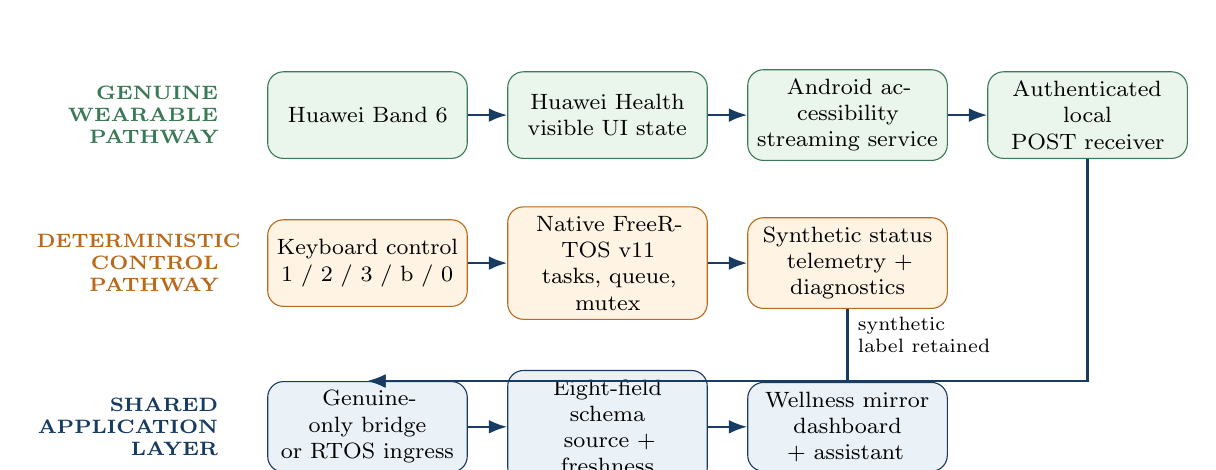
\begin{tikzpicture}[font=\footnotesize, node distance=5mm and 5mm, >=Latex,
 lane/.style={draw,rounded corners=2mm,align=center,minimum height=11mm,text width=23mm},
 genuine/.style={lane,draw=kinetiqGreen,fill=softGreen},
 synth/.style={lane,draw=kinetiqOrange,fill=softOrange},
 common/.style={lane,draw=kinetiqBlue,fill=softBlue},
 label/.style={align=right,text width=23mm,font=\scriptsize\bfseries},
 flow/.style={->,thick,draw=kinetiqBlue}]
\node[label,text=kinetiqGreen] (glabel) {GENUINE\\WEARABLE PATHWAY};
\node[genuine,right=of glabel] (band) {Huawei Band 6};
\node[genuine,right=of band] (health) {Huawei Health\\visible UI state};
\node[genuine,right=of health] (access) {Android accessibility\\streaming service};
\node[genuine,right=of access] (post) {Authenticated local\\POST receiver};
\draw[flow] (band)--(health);
\draw[flow] (health)--(access);
\draw[flow] (access)--(post);

\node[label,text=kinetiqOrange,below=9mm of glabel] (rlabel) {DETERMINISTIC\\CONTROL PATHWAY};
\node[synth,right=of rlabel] (keys) {Keyboard control\\1 / 2 / 3 / b / 0};
\node[synth,right=of keys] (native) {Native FreeRTOS v11\\tasks, queue, mutex};
\node[synth,right=of native] (rtosjson) {Synthetic status\\telemetry + diagnostics};
\draw[flow] (keys)--(native);
\draw[flow] (native)--(rtosjson);

\node[label,text=kinetiqBlue,below=11mm of rlabel] (clabel) {SHARED\\APPLICATION LAYER};
\node[common,right=of clabel] (bridge) {Genuine-only bridge\\or RTOS ingress};
\node[common,right=of bridge] (schema) {Eight-field schema\\source + freshness};
\node[common,right=of schema] (mirror) {Wellness mirror\\dashboard + assistant};
\draw[flow] (post.south) |- (bridge.north);
\draw[flow] (rtosjson.south) |- node[pos=.18,right,font=\scriptsize,align=left]{synthetic\\label retained} (bridge.north);
\draw[flow] (bridge)--(schema);
\draw[flow] (schema)--(mirror);
\end{tikzpicture}
\caption{Overall KINETIQ architecture. The two source lanes converge only after their origin and eligibility are made explicit.}
\label{fig:overall-architecture}
\end{figure}

\section{Genuine Wearable-Data Pathway}
The genuine route starts at Huawei Band 6 observations displayed through Huawei Health. A phone-side service labelled \textit{KinetiQ Streamer} reads the relevant UI state under Android accessibility permission and submits a local POST payload. The local receiver records the incoming source, schema version, timestamp, value modes, device model, simulation status, transport, and steps. A receiver record is evidence of arrival at that receiver; it is not by itself evidence that a later browser tab displayed the same value.

The genuine-only bridge examines the relay snapshot before writing the shared schema to the mirror process. It requires complete HR, SpO\textsubscript{2}, and steps values; acceptable ranges; non-simulated origin; and the relay's \code{live} freshness classification. The bridge maps activity to \code{unknown}, motion intensity to \code{0}, PPG quality to \code{good} after an upstream completed SpO\textsubscript{2} reading, and exertion through the bridge's documented heuristic. Those mappings are compatibility values, not independently measured activity, motion, PPG signal quality, or exertion. Stress may be present in the relay record, but it is not a member of the locked eight-field mirror contract and is not forwarded by the examined bridge.

\section{Deterministic FreeRTOS Control Pathway}
The native control application is a FreeRTOS v11 Windows-simulator executable. It creates four application tasks around an eight-sample queue and a mutex-protected shared control state. The console task reads operator commands approximately every 50 ms. The sensor task produces virtual IMU and DHT-like input at 100 ms intervals. The classification task drains samples and applies activity hysteresis at a nominal 1 Hz. The higher-priority telemetry task publishes one synthetic JSON status at a nominal 1 Hz and is the sole standard-output writer.

\begin{table}[H]
\centering
\small
\caption{Native FreeRTOS task structure in the examined implementation.}
\label{tab:rtos-tasks}
\begin{tabularx}{\textwidth}{p{33mm}p{22mm}p{23mm}Y}
\toprule
\textbf{Task} & \textbf{Nominal cadence} & \textbf{Priority} & \textbf{Role}\\
\midrule
Console & about 50 ms poll & idle + 1 & Reads rest, walk, run, fall, and automatic commands; updates protected control state.\\
Sensor & 100 ms & 2 & Generates virtual IMU/DHT-like samples; sends them to an eight-slot queue.\\
Classify & 1 s & 2 & Drains queue and applies state/hysteresis logic.\\
Telemetry & 1 s & 3 & Builds synthetic contract telemetry; reports timing, queue HWM, drops, and missed deadlines.\\
\bottomrule
\end{tabularx}
\end{table}

The fall command is a control event in this simulator. It must not be interpreted as a validated fall-detection algorithm or a physical sensor result. The queue is configured to retain the newest virtual inputs when pressure occurs by dropping the oldest entry, with high-water mark and dropped-event counters exposed in diagnostics.

\section{Telemetry Validation and Freshness Workflow}
Figure~\ref{fig:validation-flow} depicts the shared decision flow. Syntax alone is insufficient. Authentication applies to the receiver route; schema, complete-field, range, source, and freshness checks determine bridge or dashboard acceptance. A valid value that ceases to arrive is not kept in a live state indefinitely. The web layer tracks receiver arrival and fingerprint changes and transitions between \texttt{LIVE}, \texttt{UNCHANGED}, \texttt{STALE}, and \texttt{OFFLINE}; the documented values are blanked once offline.

\begin{figure}[H]
\centering
\resizebox{0.94\textwidth}{!}{%
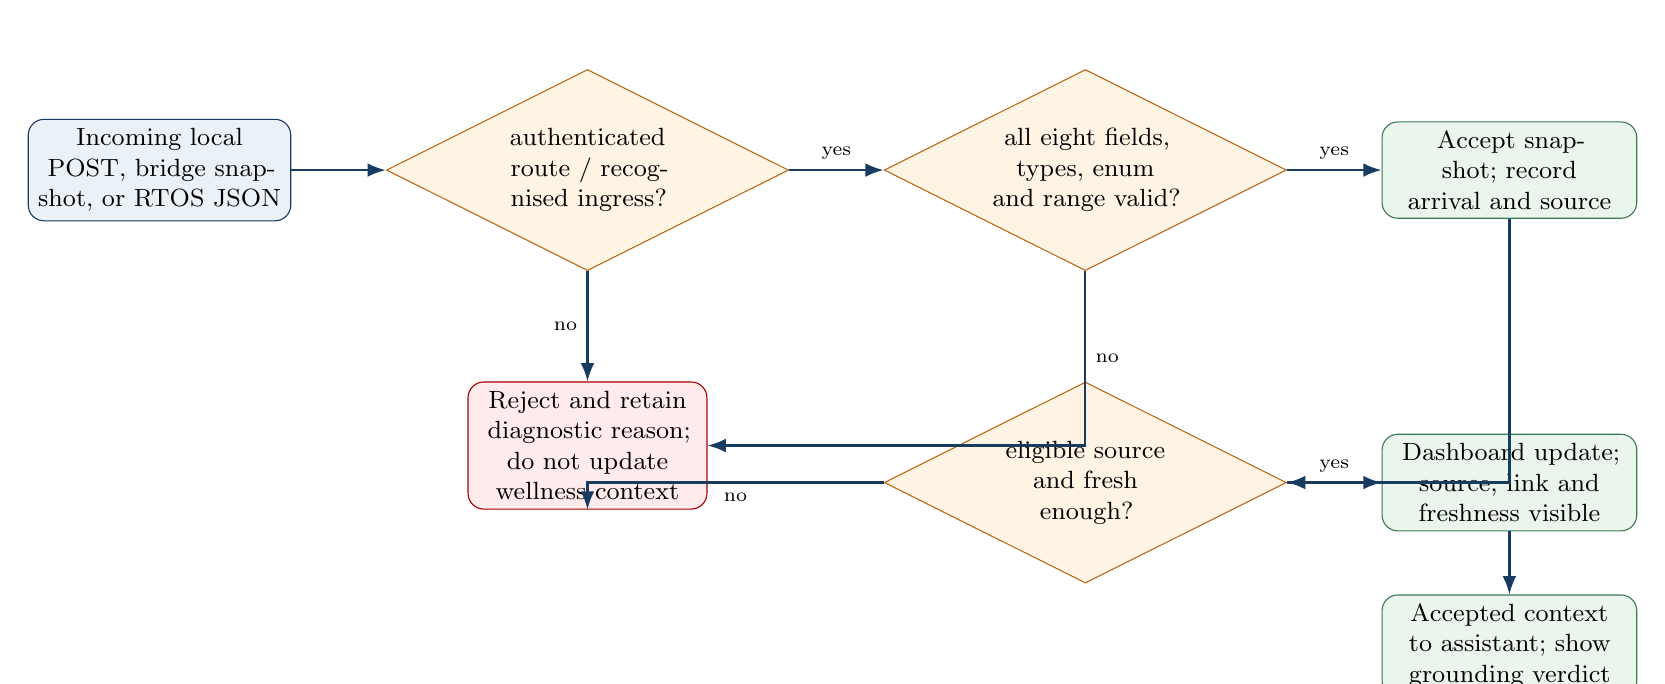
\begin{tikzpicture}[font=\small,node distance=8mm and 12mm,>=Latex,
 process/.style={draw=kinetiqBlue,fill=softBlue,rounded corners=2mm,align=center,minimum height=9mm,text width=31mm},
 decision/.style={diamond,draw=kinetiqOrange,fill=softOrange,align=center,aspect=2,text width=24mm,inner sep=1mm},
 outcome/.style={draw=kinetiqGreen,fill=softGreen,rounded corners=2mm,align=center,minimum height=9mm,text width=30mm},
 reject/.style={draw=red!65!black,fill=red!8,rounded corners=2mm,align=center,minimum height=9mm,text width=28mm},
 flow/.style={->,thick,draw=kinetiqBlue}]
\node[process] (in) {Incoming local POST, bridge snapshot, or RTOS JSON};
\node[decision,right=of in] (auth) {authenticated route / recognised ingress?};
\node[decision,right=of auth] (schema) {all eight fields, types, enum and range valid?};
\node[decision,below=14mm of schema] (source) {eligible source and fresh enough?};
\node[outcome,right=of schema] (accept) {Accept snapshot; record arrival and source};
\node[outcome,right=of source] (dash) {Dashboard update; source, link and freshness visible};
\node[outcome,below=of dash] (assist) {Accepted context to assistant; show grounding verdict};
\node[reject,below=14mm of auth] (reject) {Reject and retain diagnostic reason; do not update wellness context};
\draw[flow] (in)--(auth);
\draw[flow] (auth)-- node[above,font=\scriptsize]{yes} (schema);
\draw[flow] (auth)-- node[left,font=\scriptsize]{no} (reject);
\draw[flow] (schema)-- node[above,font=\scriptsize]{yes} (accept);
\draw[flow] (schema)|- node[pos=.25,right,font=\scriptsize]{no} (reject);
\draw[flow] (accept) |- (source);
\draw[flow] (source)-- node[above,font=\scriptsize]{yes} (dash);
\draw[flow] (source)-| node[pos=.25,below,font=\scriptsize]{no} (reject);
\draw[flow] (dash)--(assist);
\end{tikzpicture}}
\caption{Validation and freshness workflow. The genuine bridge adds source-specific completeness and live-freshness guards before it emits the shared contract.}
\label{fig:validation-flow}
\end{figure}

\section{Dashboard and Assistance Layer}
The laptop dashboard runs a threaded HTTP server on loopback, tries port 8777 and then 8778 when necessary, and ingests valid JSON through standard input or application endpoints. It maintains a snapshot plus arrival and value-change times. The cards show accepted wellness context along with the source and data state. Browser-camera handling is limited to a pixel-difference motion proxy; no implemented pose or posture classifier is claimed.

\begin{figure}[H]
\centering
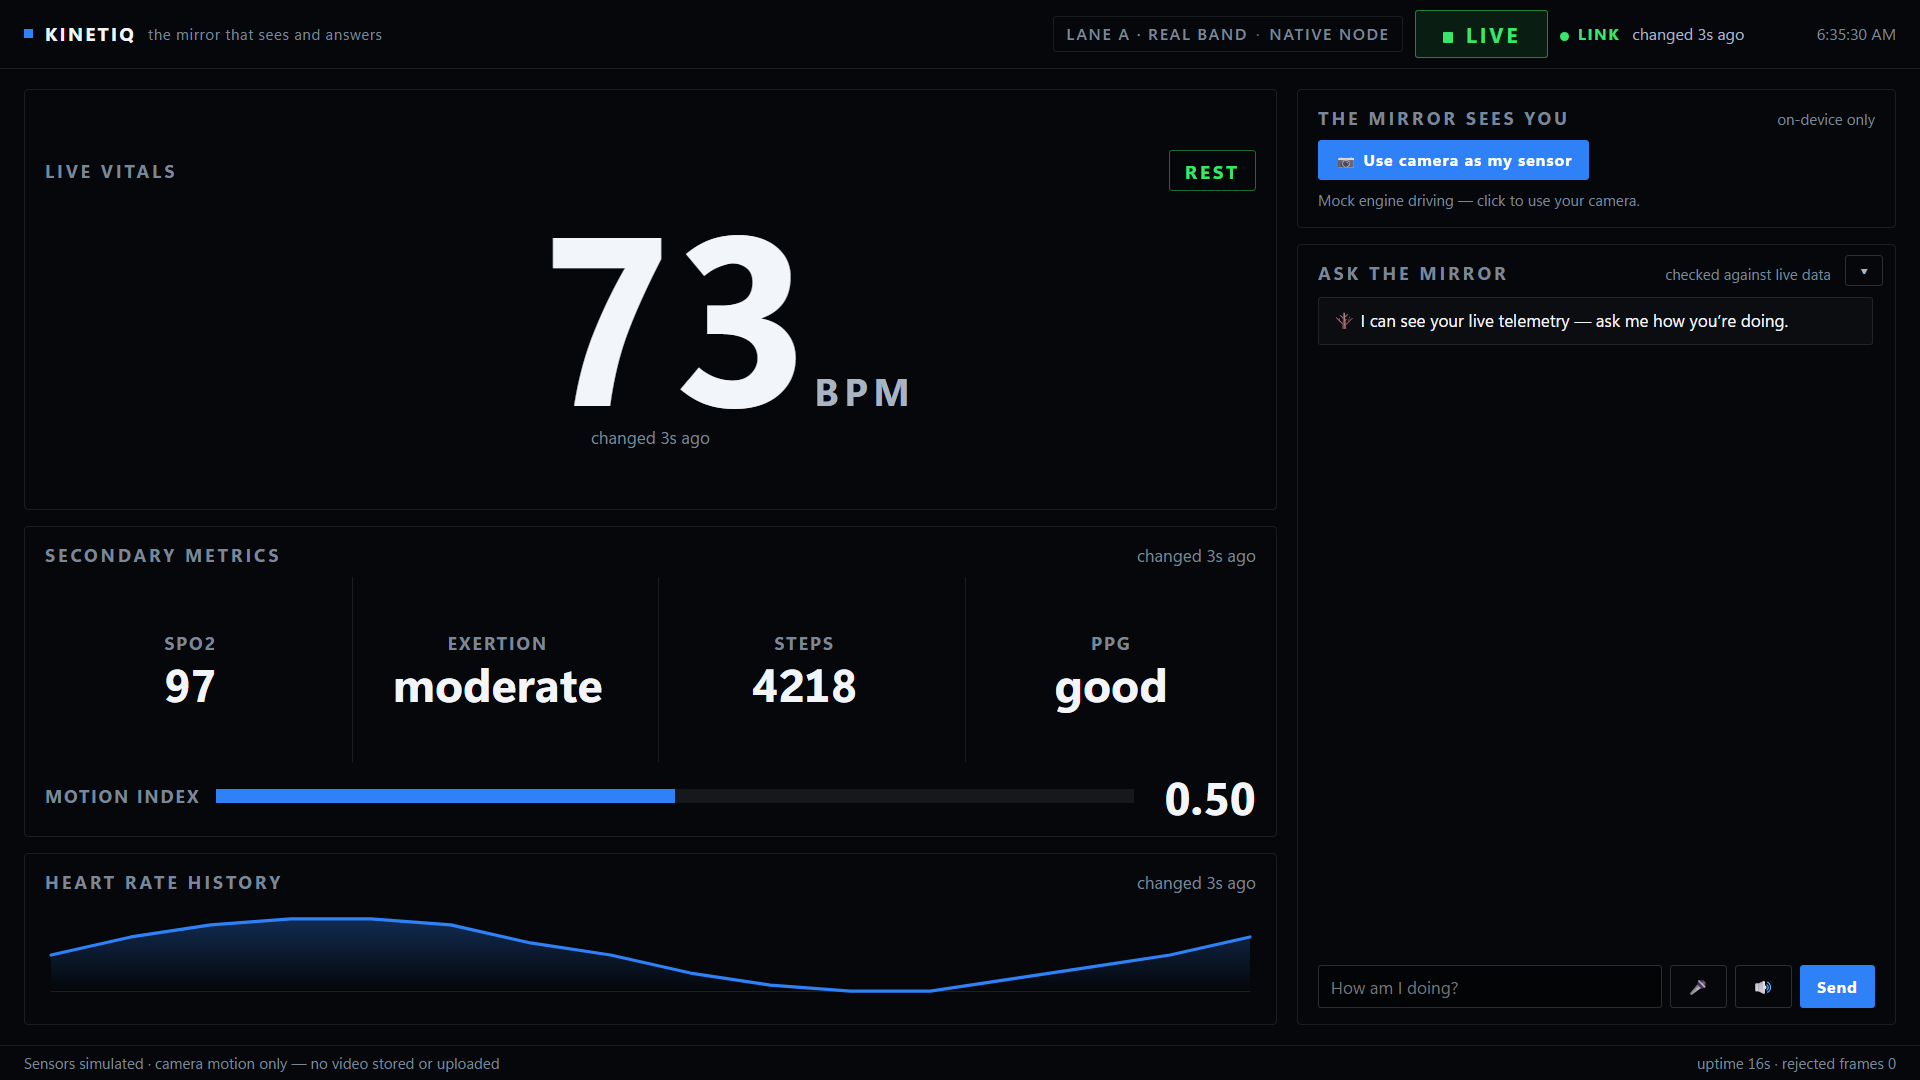
\includegraphics[width=\textwidth]{ui_live.png}
\caption[Dashboard mirror with synthetic stream (not live)]{Implemented dashboard mirror rendered in the browser during a controlled local input session; the displayed stream is synthetic, not live wearable telemetry.}
\label{fig:dashboard-live}
\end{figure}

The assistant accepts the current validated context, attempts a local Ollama \code{gemma2:2b} response where available, and otherwise uses a deterministic template. Responses are bounded to 70 words.

The verifier checks specified agreement with activity, exertion, an exact HR/heart value or step count, and poor-quality wording when applicable. The process shows \texttt{PASS} or \texttt{FAIL}; the examined implementation still sends text to speech after a failed check, so the verdict is informative rather than a fail-closed safety gate.

\section{Hardware Design Scope}
The selected embedded components are an ESP32 DevKit V1, MPU6050, HC-SR04, infrared sensor, DHT22, and supporting wiring/prototyping materials. The materials include pin mapping and a Wokwi sketch. Figure~\ref{fig:hardware-concept} reproduces the project material's earlier hardware-path diagram as a conceptual design reference. It is not used as evidence of final physical sensor acquisition.

\begin{figure}[H]
\centering
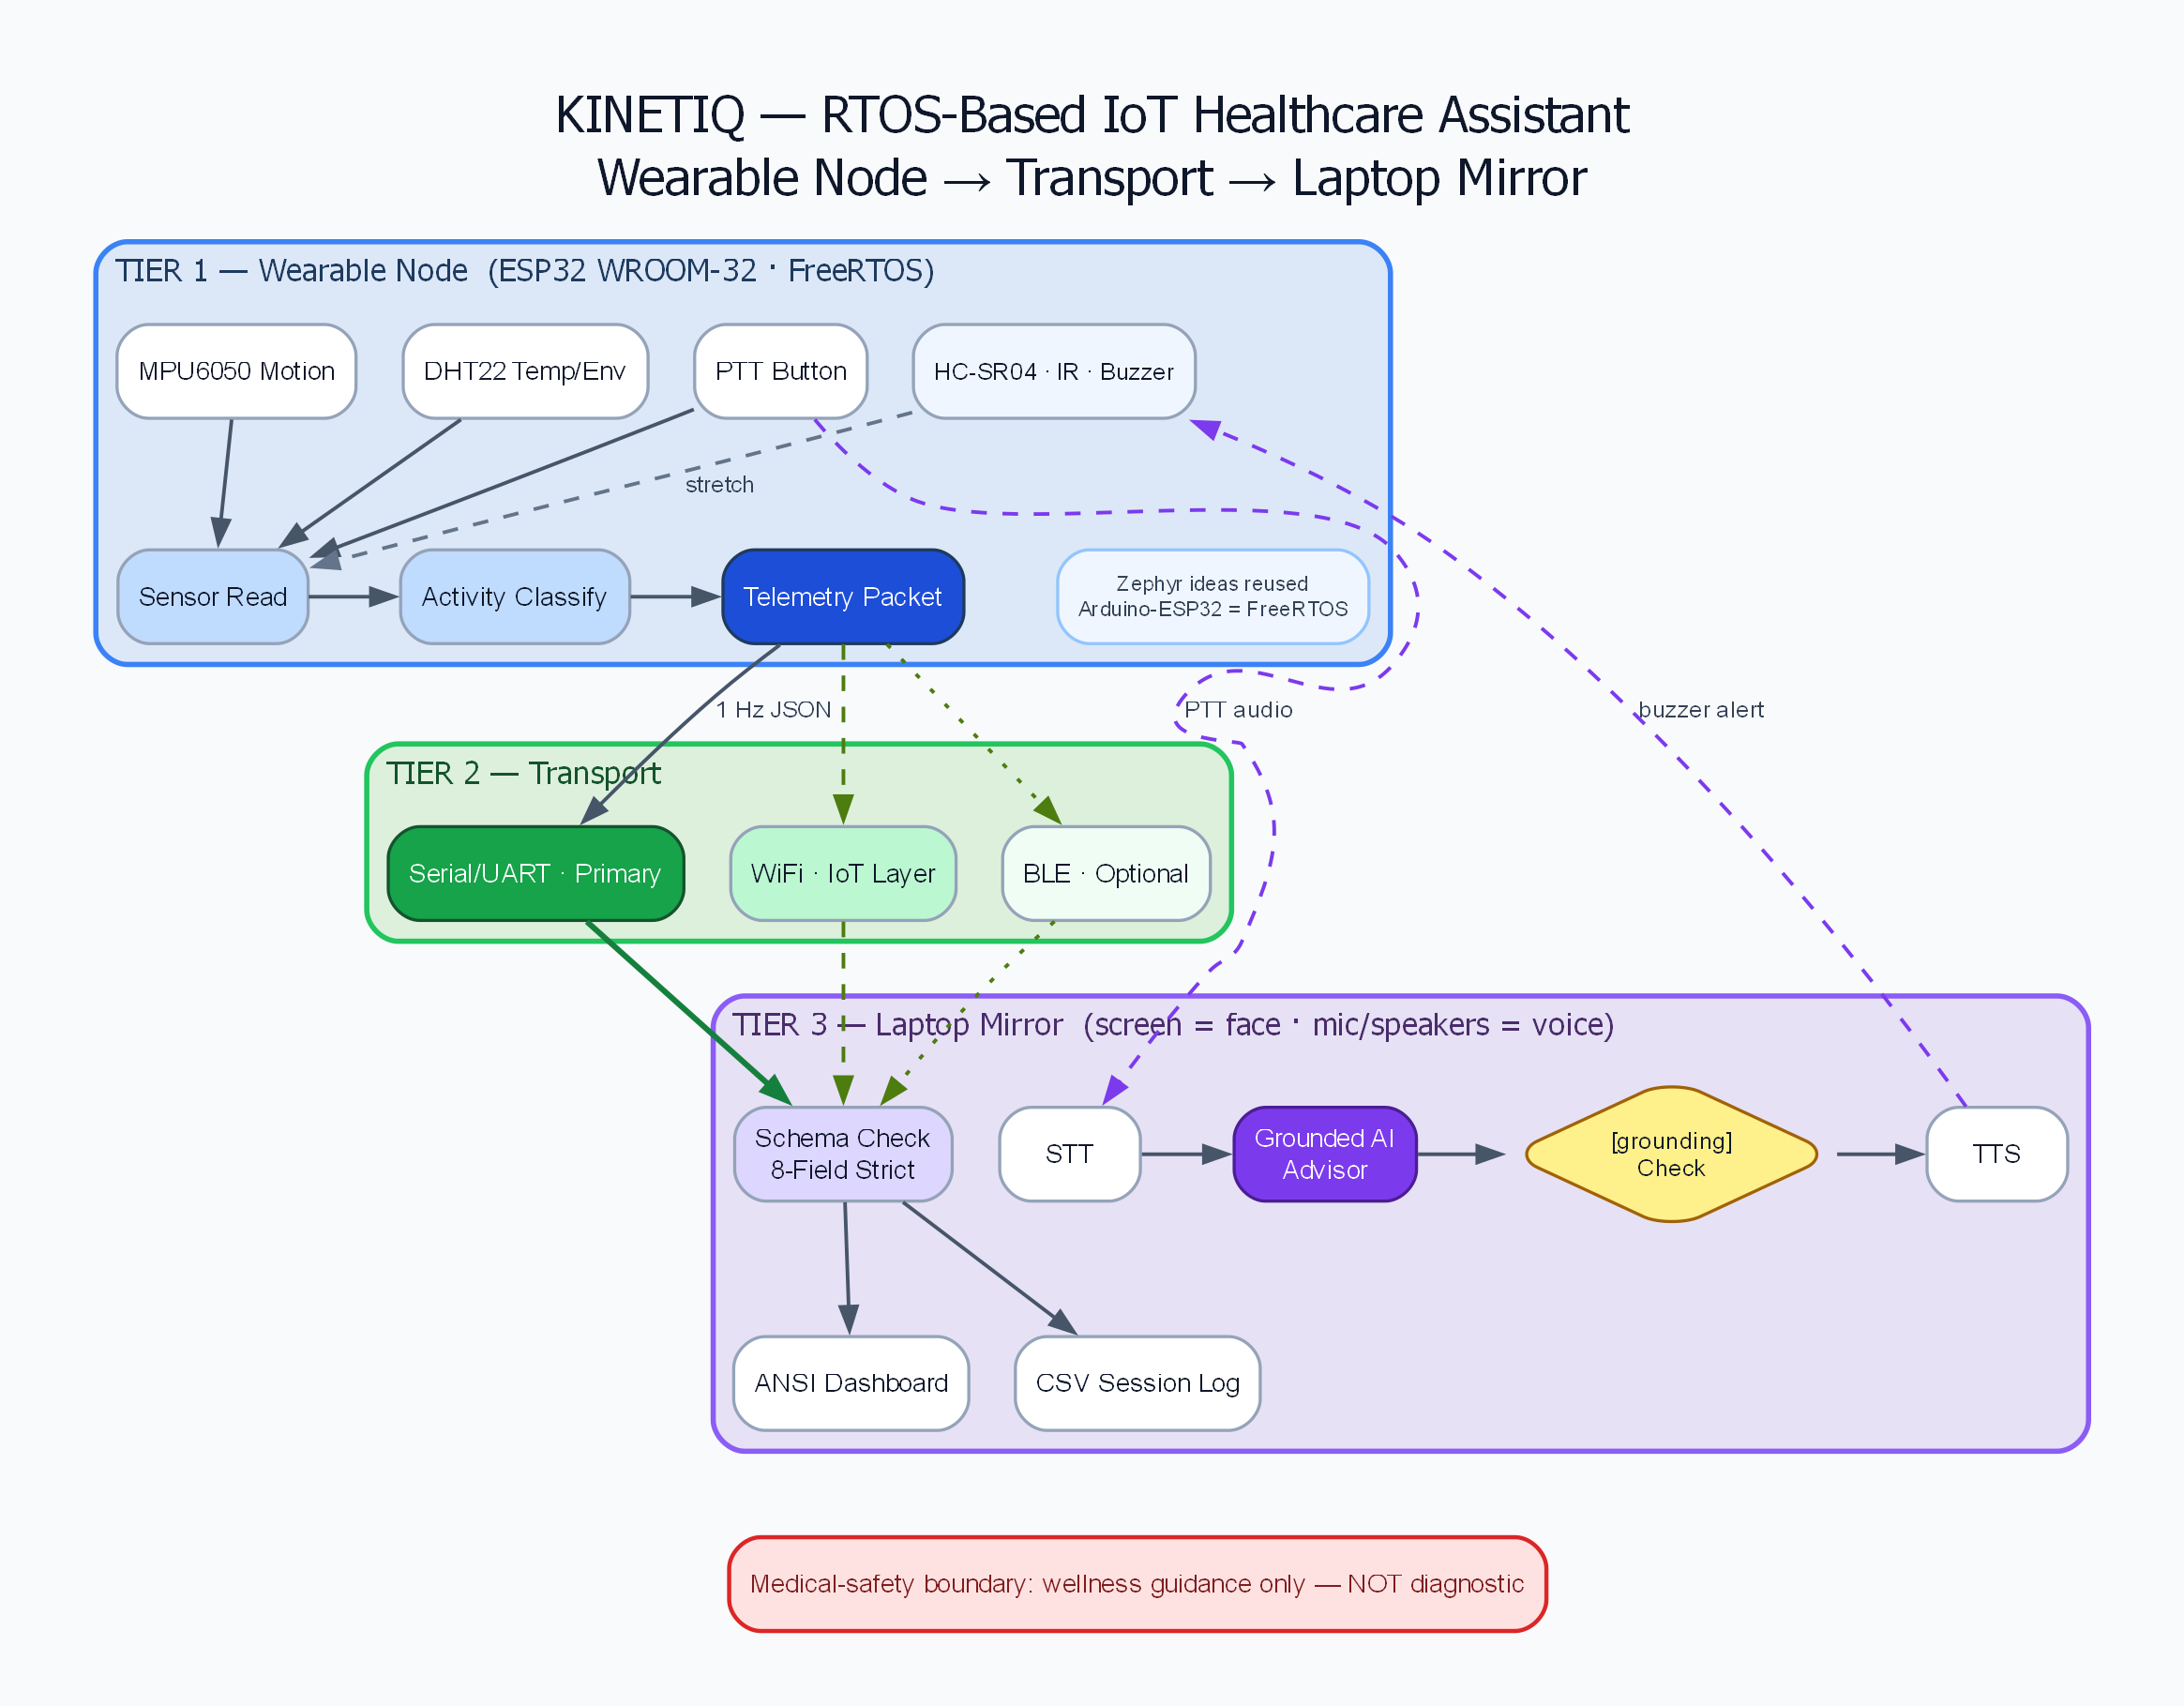
\includegraphics[width=0.82\textwidth]{existing_architecture.png}
\caption{Earlier hardware-path conceptual architecture from the KINETIQ project materials. The physical ESP32 sensing path remained planned/simulated at the documented final demonstration.}
\label{fig:hardware-concept}
\end{figure}

The ESP32 and sensor selection remains technically appropriate for a future sensing node, but physical wiring, calibration, power behaviour, environmental response, and end-to-end sensor ingestion require separate validation. Wokwi execution can exercise the modelled sketch, not replace those measurements.

\chapter{IMPLEMENTATION AND METHODOLOGY}

\section{Software Organisation}
The implementation is organised as cooperating, deliberately narrow modules. The native FreeRTOS source at \code{hardware/native/}\allowbreak\code{kinetiq\_tasks.c} produces synthetic control messages and diagnostics. The Python receiver package contains the shared schema, BLE mock, bridge-related helpers, and local data handling. The web application at \code{laptop/web/}\allowbreak\code{app.py} owns dashboard state and exposes local endpoints. The AI and voice modules reside under \code{laptop/ai}. This separation keeps a transport adapter from becoming an unexamined source of truth for the UI.

\begin{table}[H]
\centering
\small
\caption{Principal implementation modules and responsibilities.}
\label{tab:modules}
\begin{tabularx}{\textwidth}{p{43mm}Yp{30mm}}
\toprule
\textbf{Module} & \textbf{Responsibility} & \textbf{Evidence category}\\
\midrule
\code{kinetiq\_tasks.c} & FreeRTOS task creation, synthetic samples, activity state, queue/mutex use, timing and JSON telemetry. & Implemented native control runtime\\
\code{telemetry\_schema.py} & Required-key, type, range, and enumeration validation for common payloads. & Implemented shared validation\\
\code{band\_bridge.py} & Maps eligible relay snapshots to the locked mirror schema; blocks simulated, incomplete, non-live, and out-of-range input. & Implemented bridge logic\\
\code{app.py} & Loopback dashboard server, state ageing, valid JSON ingestion, API routes, session context. & Implemented local application\\
\code{assistant.py} & Context prompt/template, response word limit, grounding checker, TTS invocation. & Implemented assistant logic\\
\code{voice\_pipeline.py} & Local faster-whisper transcription path and audio compatibility handling. & Implemented voice module\\
\code{hardware/sim} & Wokwi sketch and supporting simulation configuration. & Simulation/design evidence\\
\bottomrule
\end{tabularx}
\end{table}

\section{FreeRTOS Tasks, Queue, and Synchronisation}
The control node initialises an eight-element sample queue and a mutex for the shared control state, then creates console, sensor, classification, and telemetry tasks. The sensor task produces virtual sensor samples at 100 ms. The classification task consumes queued samples once per second and uses hysteresis to reduce rapid state changes. A higher-priority telemetry task publishes a one-second status payload. Standard output ownership is confined to the telemetry task, which prevents interleaved JSON fragments from multiple writers.

Timing diagnostics use a monotonic high-resolution counter on the host. For each periodic release the code records intended period, measured period, maximum lateness, queue high-water mark, dropped events, and missed deadlines. A documented lateness threshold of 120 ms contributes to the missed-deadline diagnostic. These figures aid repeatable debugging of the desktop simulator; they do not establish a scheduling bound on every Windows execution.

\begin{figure}[H]
\centering
\resizebox{0.96\textwidth}{!}{%
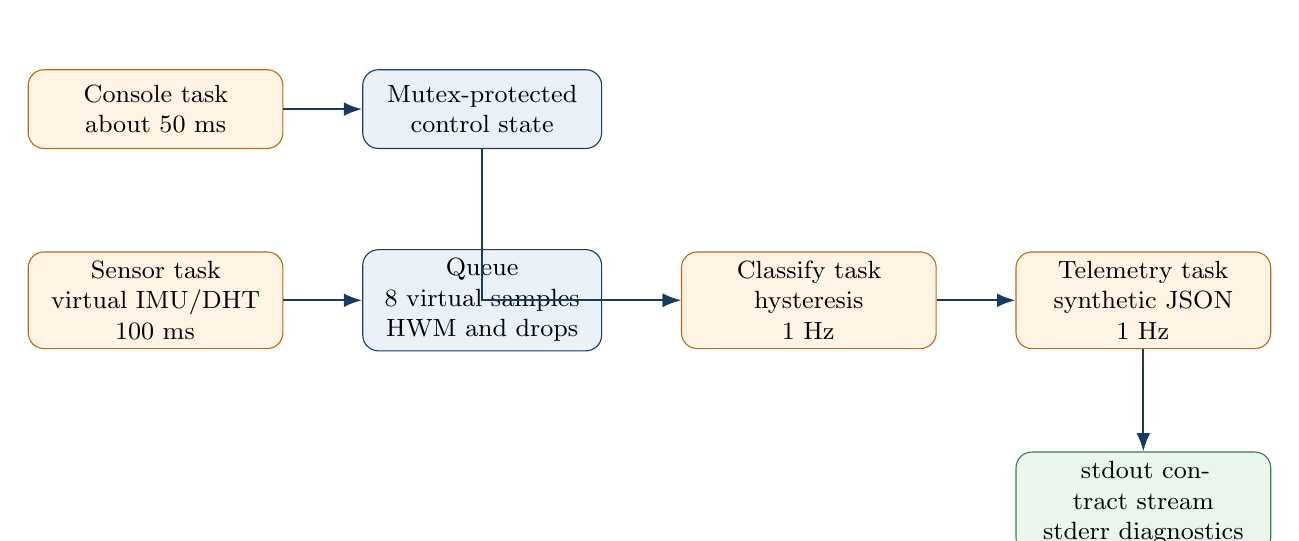
\begin{tikzpicture}[font=\small,node distance=9mm and 10mm,>=Latex,
 task/.style={draw=kinetiqOrange,fill=softOrange,rounded corners=2mm,align=center,minimum height=10mm,text width=30mm},
 shared/.style={draw=kinetiqBlue,fill=softBlue,rounded corners=2mm,align=center,minimum height=10mm,text width=28mm},
 output/.style={draw=kinetiqGreen,fill=softGreen,rounded corners=2mm,align=center,minimum height=10mm,text width=30mm},
 flow/.style={->,thick,draw=kinetiqBlue}]
\node[task] (console) {Console task\\about 50 ms};
\node[shared,right=of console] (mutex) {Mutex-protected\\control state};
\node[task,below=13mm of console] (sensor) {Sensor task\\virtual IMU/DHT\\100 ms};
\node[shared,right=of sensor] (queue) {Queue\\8 virtual samples\\HWM and drops};
\node[task,right=of queue] (classify) {Classify task\\hysteresis\\1 Hz};
\node[task,right=of classify] (telemetry) {Telemetry task\\synthetic JSON\\1 Hz};
\node[output,below=13mm of telemetry] (out) {stdout contract stream\\stderr diagnostics};
\draw[flow] (console)--(mutex);
\draw[flow] (mutex)|- (classify);
\draw[flow] (sensor)--(queue);
\draw[flow] (queue)--(classify);
\draw[flow] (classify)--(telemetry);
\draw[flow] (telemetry)--(out);
\end{tikzpicture}}
\caption{Native FreeRTOS control data path. All values emitted here are synthetic RTOS-control telemetry.}
\label{fig:rtos-dataflow}
\end{figure}

\section{Genuine-Path Ingestion and Bridging}
The Android relay converts relevant Huawei Health interface observations into a local payload. The authenticated receiver persists each accepted relay row with source and transport metadata. The bridge then uses an all-or-nothing policy for the mirror's required physiological fields: HR, SpO\textsubscript{2}, and steps must all exist and pass range checks. Relay freshness must be \code{live}, and \code{simulated} must be false. Any failed precondition blocks forwarding.

The following pseudocode captures the bridge decision without exposing application secrets or unrelated implementation detail:

\begin{lstlisting}[caption={Genuine-only bridge policy, simplified.},label={lst:bridge-policy}]
snapshot = read_latest_authenticated_relay_snapshot()
if snapshot.simulated or snapshot.freshness != "live": reject()
if missing(snapshot.hr, snapshot.spo2, snapshot.steps): reject()
if not in_range(snapshot.hr, 30, 220): reject()
if not in_range(snapshot.spo2, 70, 100): reject()
if snapshot.steps < 0: reject()

emit_to_mirror({timestamp, heart_rate, spo2, activity="unknown",
  motion_intensity=0, exertion=bridge_heuristic(...),
  steps, ppg_quality="good"})
\end{lstlisting}

The PPG-quality assignment is an upstream-completion proxy, not a signal-quality algorithm. The exertion field is a bridge heuristic. The reporting language therefore treats the bridge output as validated transport context with selected derived fields, not as a fully measured physiological model.

\section{Schema Validation and Dashboard State}
The web ingress parses JSON, validates the eight required keys, and ignores non-JSON standard-input lines. The validator restricts activity to \code{rest}, \code{walk}, \code{run}, \code{active}, or \code{unknown}; exertion to \code{rest}, \code{light}, \code{moderate}, or \code{high}; and PPG quality to \code{good} or \code{poor}. Numeric boundaries are listed in Table~\ref{tab:telemetry-contract}. Rejected packets do not replace the accepted wellness snapshot.

Freshness is implemented in the web layer with a 60 s live interval, a subsequent 60 s stale interval, and an offline limit at 300 s. The code additionally detects whether a newly arriving packet changed the snapshot fingerprint. This distinguishes a recently arriving repeated value (\texttt{UNCHANGED}) from a value that has stopped arriving (\texttt{STALE} or \texttt{OFFLINE}). The value display is blanked in the offline condition.

\begin{table}[H]
\centering
\small
\caption{Dashboard freshness and link-state treatment.}
\label{tab:freshness-states}
\begin{tabularx}{\textwidth}{p{35mm}p{36mm}Y}
\toprule
\textbf{State} & \textbf{Condition in examined UI logic} & \textbf{Interface consequence}\\
\midrule
LIVE & Recent arrival with a changed fingerprint inside the live interval. & Current card and source state are displayed.\\
UNCHANGED & Recent arrival but repeated fingerprint. & Card remains visible; repetition is not disguised as a changed sample.\\
STALE & Arrival age exceeds the live interval but remains below offline threshold. & Stale status is visible.\\
OFFLINE & Arrival age exceeds 300 s. & Documented interface blanks measurement values and shows offline state.\\
\bottomrule
\end{tabularx}
\end{table}

\section{Grounded Assistance and Voice Route}
The assistant constructs a local context containing accepted telemetry fields and generates through an optional local Ollama \code{gemma2:2b} endpoint. When that endpoint is unavailable, a deterministic template remains available. The response is limited to 70 words. The verifier inspects required contextual mentions: activity and exertion normally appear in the response; an exact heart-rate/heart wording or exact step count relaxes the requirement for both; and poor PPG quality requires qualifying language. The result is surfaced as \texttt{PASS} or \texttt{FAIL} in the application.

Speech input is transcribed through faster-whisper \code{tiny.en} with \code{int8} inference. Text-to-speech is invoked for the generated answer. A synthetic-clip result measures the transcription route in a controlled condition only. Browser camera input, where used, supplies a motion proxy based on frame-pixel differences and is not a body-pose system.

\section{Launch and Fallback Procedure}
The reproducible operator route is deliberately simple:

\begin{enumerate}
  \item start the local web application and confirm its loopback port;
  \item start the authenticated receiver and either the genuine-only bridge or the native FreeRTOS control executable;
  \item inspect the dashboard source and freshness card before discussing a value;
  \item use a fresh complete Huawei relay snapshot only when a genuine-path demonstration is required;
  \item select the RTOS lane when transport is unavailable, retaining its synthetic label; and
  \item retain console diagnostics and CSV/session artefacts for the demonstration record.
\end{enumerate}

The fallback retains operability, not equivalence: RTOS synthetic values cannot substitute for unavailable wearable observations.

\section{Hardware Simulation and Integration Status}
The Wokwi sketch models the embedded direction with task-oriented code and simulated inputs. It supports early pin and logic exploration. The selected physical BOM and pin map support planned assembly, but the final documented demonstration does not claim newly acquired ESP32 readings. No section of the runtime validation should be interpreted as a completed physical MPU6050, HC-SR04, infrared, or DHT22 integration.

\chapter{RESULTS AND DISCUSSION}

\section{Evidence Classification}
The results are classified by pathway and test condition before interpretation. A receiver CSV row, a mock stream, a simulator diagnostic, and a physical sensor trace have different evidential meaning. Table~\ref{tab:evidence-classification} prevents a successful bounded test from being presented as a broader system claim.

\begin{table}[H]
\centering
\small
\caption{Evidence classification used for reported observations.}
\label{tab:evidence-classification}
\begin{tabularx}{\textwidth}{p{39mm}p{45mm}Y}
\toprule
\textbf{Evidence} & \textbf{What it establishes} & \textbf{What it does not establish}\\
\midrule
Huawei relay receiver row & A relay payload reached and was stored by the authenticated local receiver. & Browser display of every row; clinical validity; direct Huawei API use.\\
Dashboard mock CSV & A synthetic stream was processed under its recorded run condition. & Live wearable throughput or clinical telemetry performance.\\
BLE mock counter & Mock routing handled the stated message count. & Device-specific BLE pairing or Huawei Band transport.\\
FreeRTOS host diagnostics & Behaviour of the Windows-hosted control runtime. & Hard real-time guarantee or genuine physiology.\\
Wokwi sketch & Simulated hardware/control logic and planned pin pathway. & Physical sensor acquisition or calibration.\\
\bottomrule
\end{tabularx}
\end{table}

\section{Genuine Wearable-Path Observation}
The receiver log contains Huawei-Health relay entries dated 22 October 2026. One complete record stores heart rate 60 BPM, SpO\textsubscript{2} 100\%, stress 57, and 4,181 steps, identified as \code{huawei\_band\_6\_healthapp}, \code{simulated=false}, and transport \code{health\_app\_ui}. The same record classifies heart rate and stress as real-time while labelling SpO\textsubscript{2} historical. A nearby earlier record stores 74 BPM, 100\% SpO\textsubscript{2}, stress 57, and 4,181 steps. These are documented relay observations, not clinical measurements.

\begin{table}[H]
\centering
\small
\caption{Selected documented Huawei-Health relay observations at the local receiver.}
\label{tab:genuine-observations}
\begin{tabularx}{\textwidth}{p{28mm}p{18mm}p{18mm}p{17mm}p{18mm}Y}
\toprule
\textbf{Receiver time} & \textbf{HR} & \textbf{SpO\textsubscript{2}} & \textbf{Stress} & \textbf{Steps} & \textbf{Qualification}\\
\midrule
2026-10-22 13:14:35 & 74 BPM & 100\% & 57 & 4,181 & Complete relay record; health-app UI transport.\\
2026-10-22 13:17:37 & 60 BPM & 100\% & 57 & 4,181 & HR/stress marked real-time; SpO\textsubscript{2} marked historical in the stored relay metadata.\\
2026-10-23 01:58 & 78 BPM & 99\% & absent & 5,432 & Later complete HR/SpO\textsubscript{2}/steps record; stress absent.\\
\bottomrule
\end{tabularx}
\end{table}

The bridge accepts only fresh, complete HR, SpO\textsubscript{2}, and steps according to its own contract. Because stress is not a shared schema field, the recorded stress observation cannot be claimed as mirror context. The inspected materials establish receiver-side acceptance and bridge eligibility logic; they do not contain a corresponding browser capture proving that every selected row reached the mirror. The genuine result is therefore qualified as \pmark.

\section{Schema and Bridge Validation}
Integration logic covers complete live snapshots, missing HR/SpO\textsubscript{2}/steps, stale values, simulated origin, and out-of-range values. The expected acceptance mapping for a valid live snapshot includes HR 74, SpO\textsubscript{2} 100, and steps 4,181 with activity \code{unknown}, motion intensity zero, \code{good} PPG quality proxy, and heuristic exertion. The negative paths demonstrate an important safety property: malformed or ineligible genuine-lane input is blocked before it becomes an apparently current dashboard value.

No statistic for live rejection rate is reported because a controlled representative sample count and test log for that rate were not identified. The result establishes branch behaviour in the available integration test and source, not a field reliability percentage.

\section{Dashboard Mock Stream}
The recorded dashboard session \code{session\_20261014\_193826.csv} contains 75 telemetry frames over 15 seconds with zero dropped frames in the associated documented mock run. Figure~\ref{fig:mock-telemetry} retains the source chart's explicit synthetic label. The chart consists of a mock sensor stream, so its apparent time trends must not be interpreted as genuine wearable biometrics.

\begin{figure}[H]
\centering
\begin{subfigure}[t]{0.48\textwidth}
  \centering
  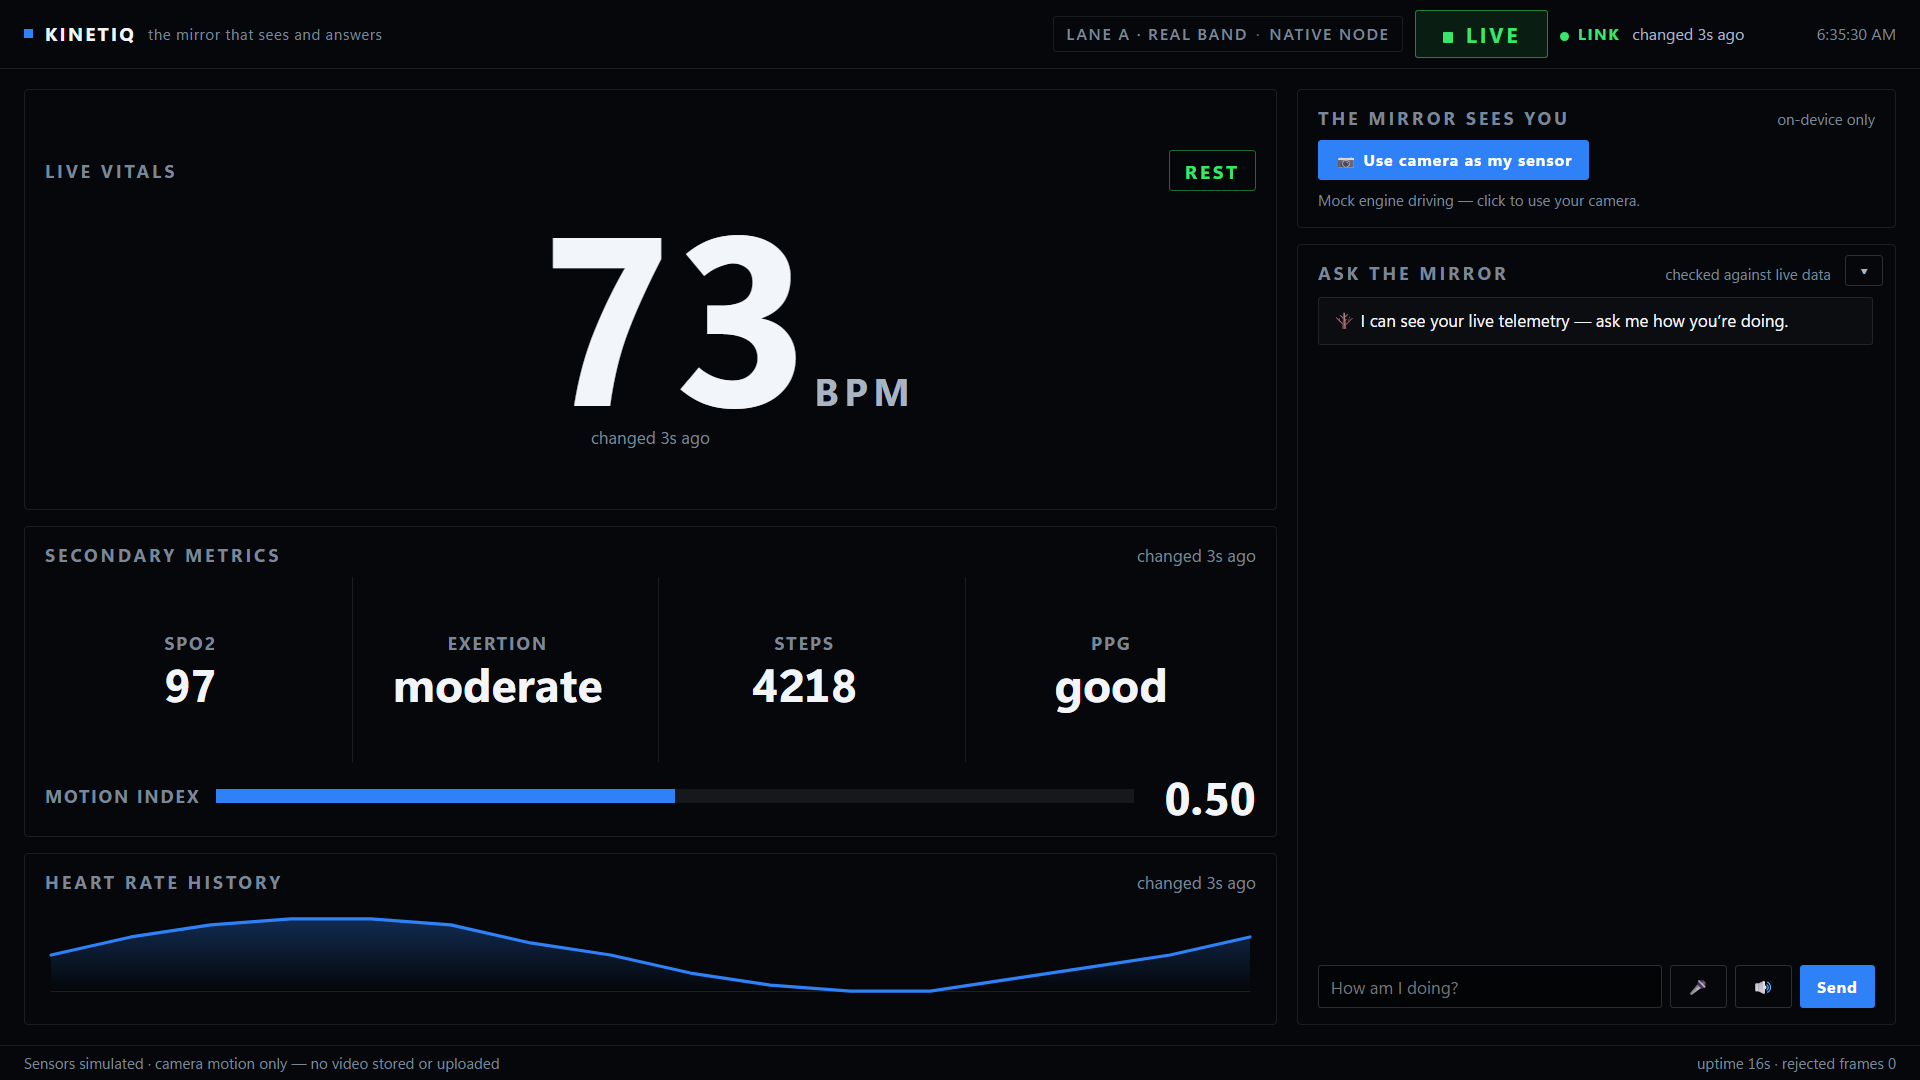
\includegraphics[width=\textwidth]{ui_live.png}
  \caption{Live}
  \label{fig:dashboard-states-live}
\end{subfigure}\hfill
\begin{subfigure}[t]{0.48\textwidth}
  \centering
  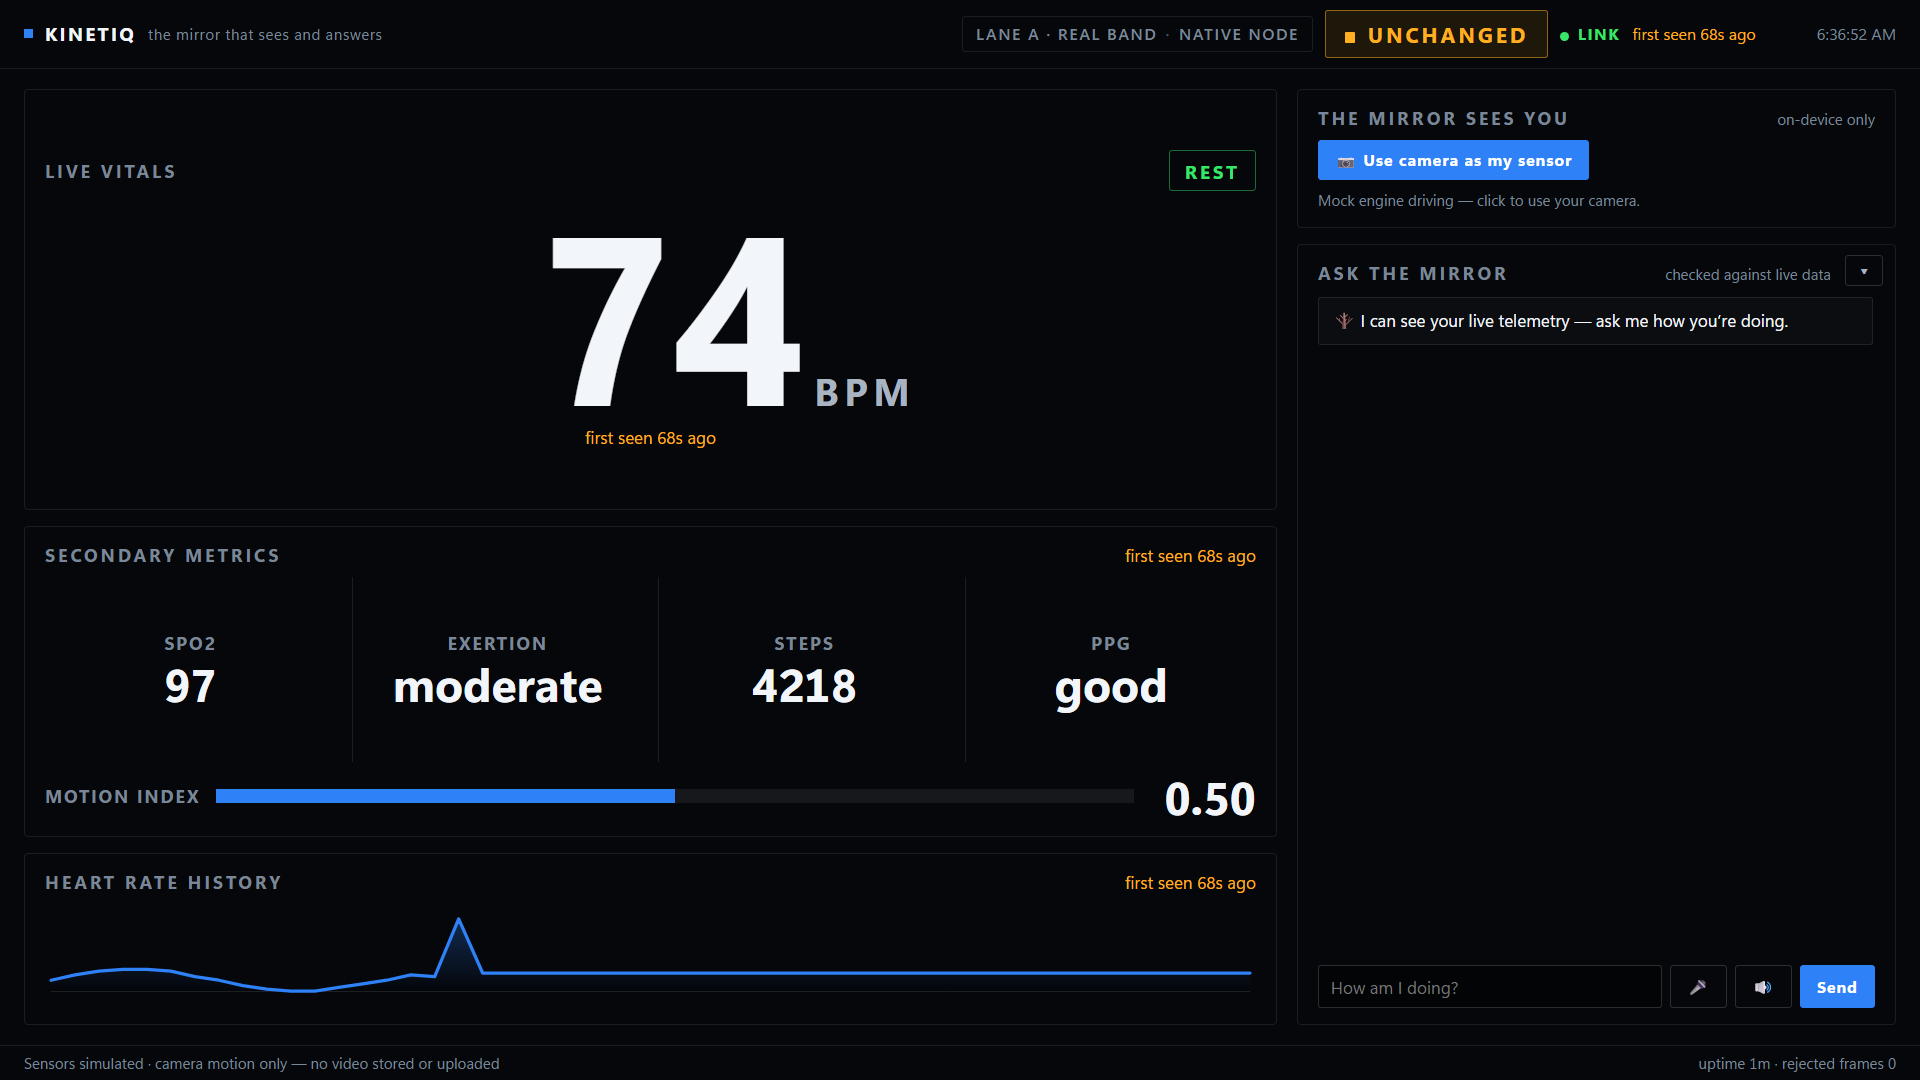
\includegraphics[width=\textwidth]{ui_unchanged.png}
  \caption{Unchanged}
  \label{fig:dashboard-states-unchanged}
\end{subfigure}\\[3pt]
\begin{subfigure}[t]{0.48\textwidth}
  \centering
  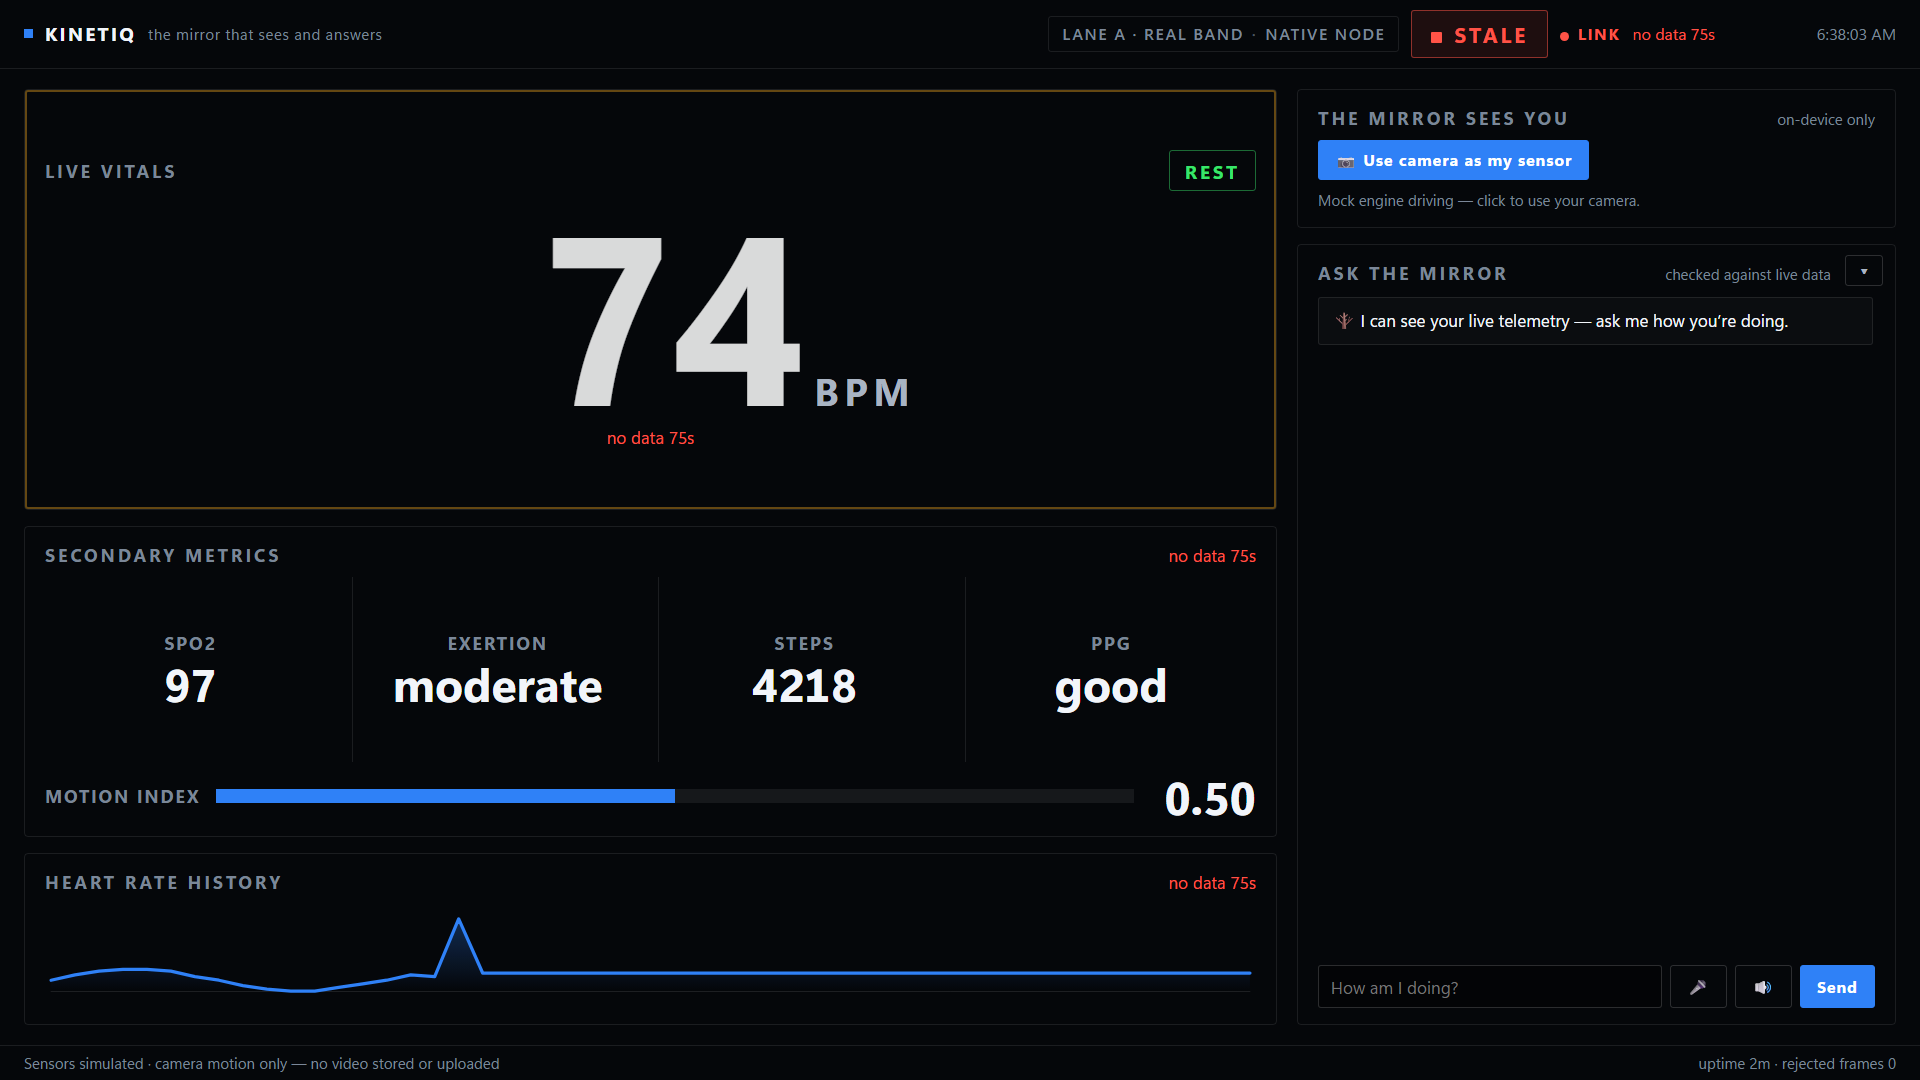
\includegraphics[width=\textwidth]{ui_stale.png}
  \caption{Stale}
  \label{fig:dashboard-states-stale}
\end{subfigure}\hfill
\begin{subfigure}[t]{0.48\textwidth}
  \centering
  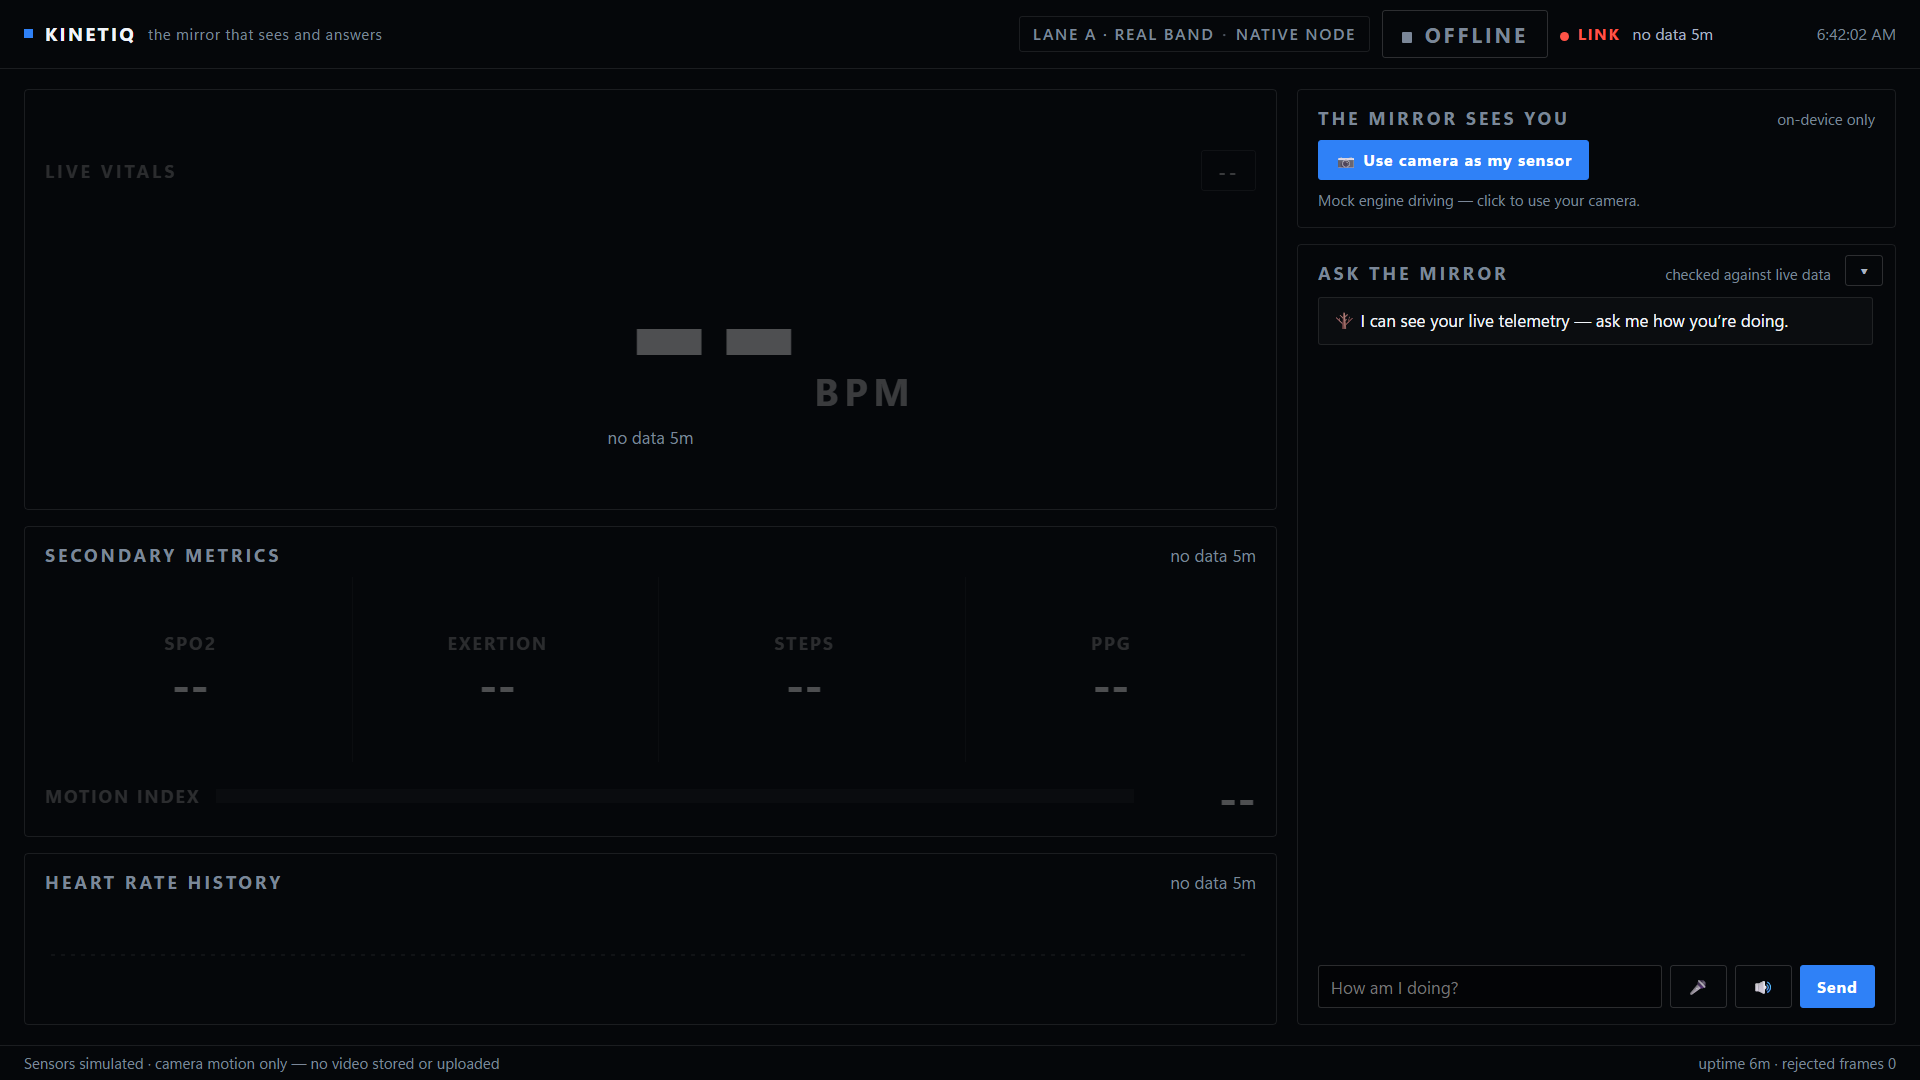
\includegraphics[width=\textwidth]{ui_offline.png}
  \caption{Offline}
  \label{fig:dashboard-states-offline}
\end{subfigure}
\caption[Dashboard freshness states (synthetic input)]{Dashboard freshness states observed under controlled synthetic input: live, unchanged, stale and offline. These captures exercise the freshness/offline logic; they are not live wearable telemetry.}
\label{fig:dashboard-states}
\end{figure}

\begin{figure}[H]
\centering
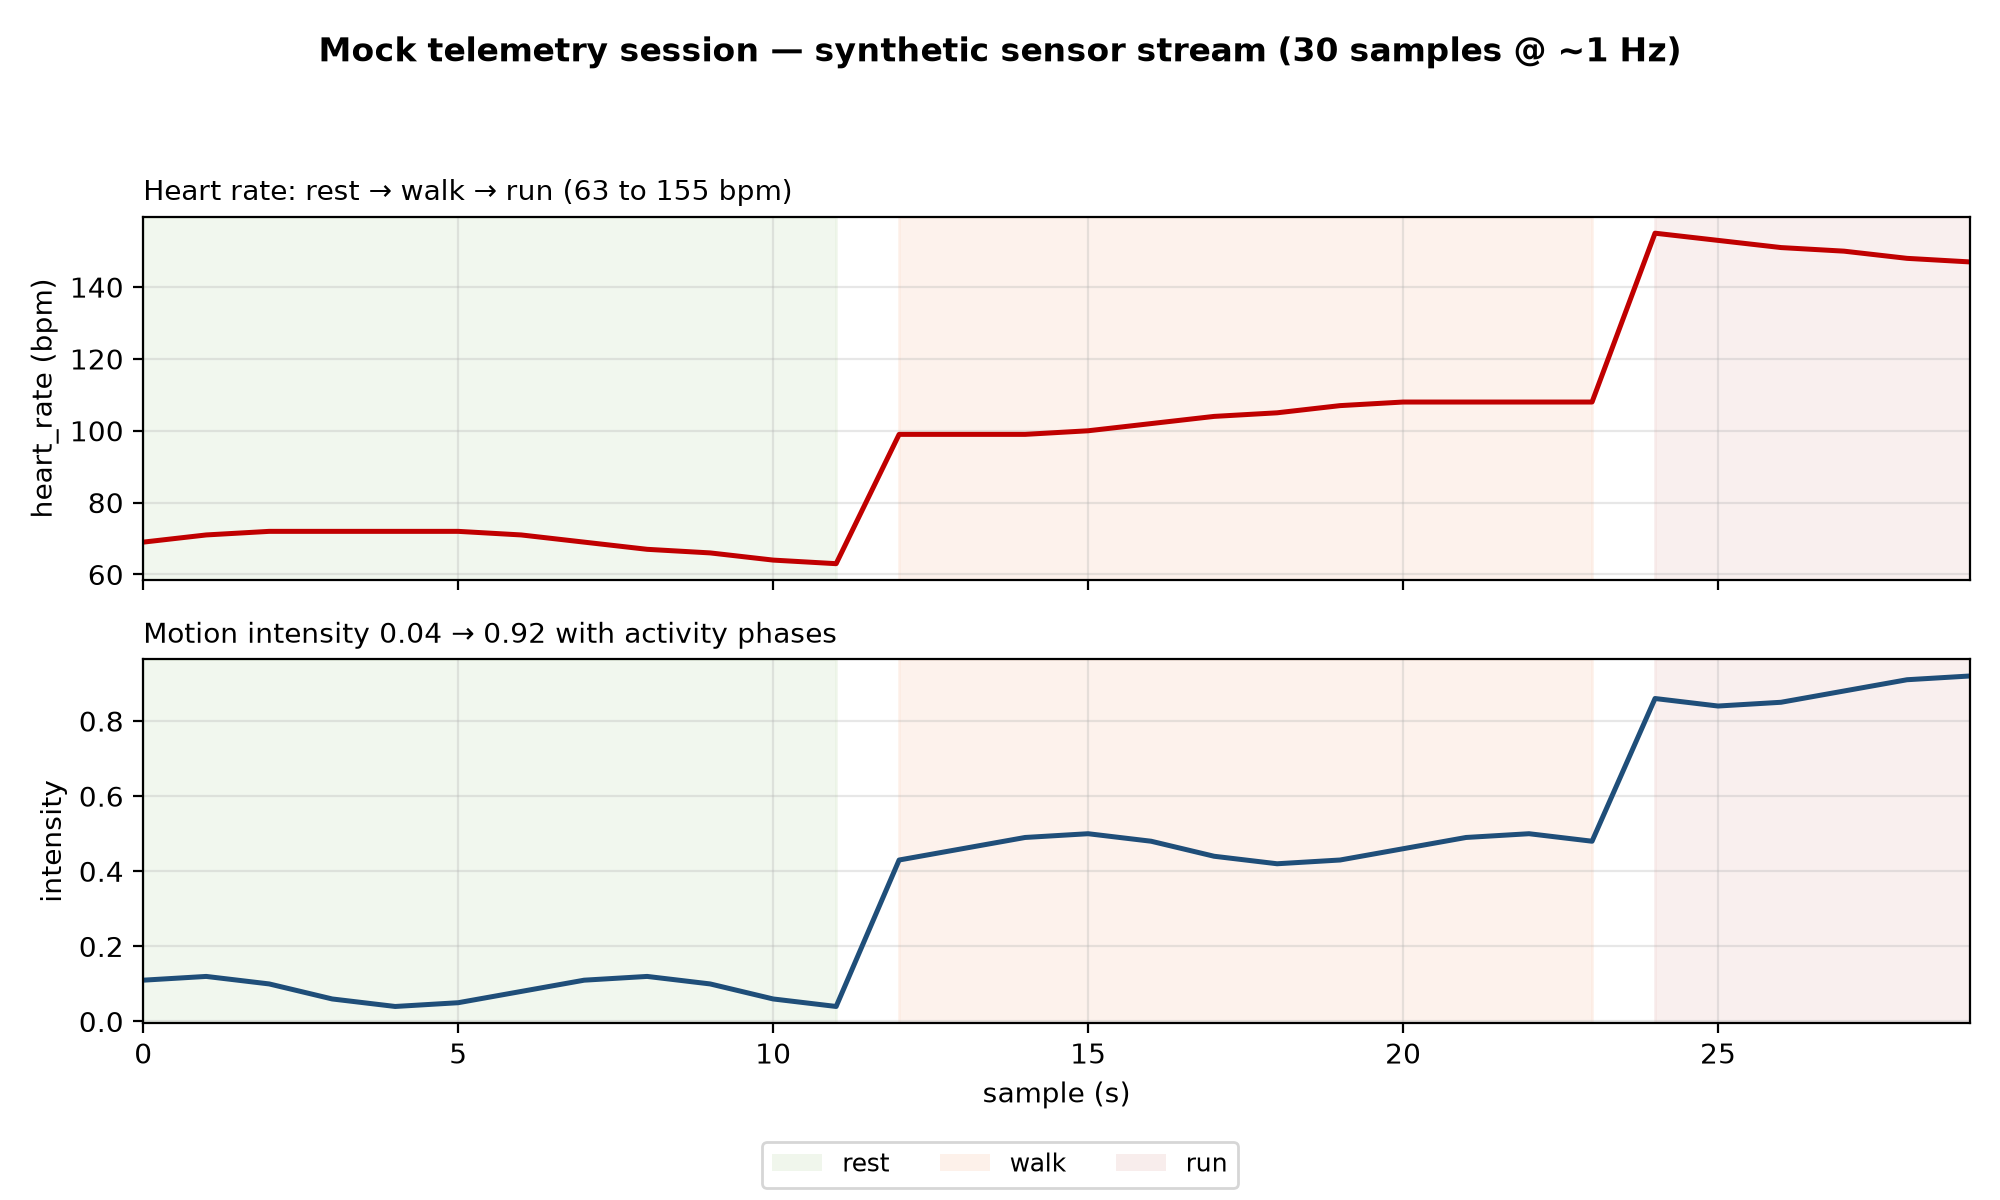
\includegraphics[width=\textwidth]{mock_telemetry_results.png}
\caption[Mock telemetry session (synthetic, 30 samples)]{Mock telemetry session: synthetic sensor stream (30 samples at approximately 1 Hz) from the project materials. It is not a genuine biometric time series.}
\label{fig:mock-telemetry}
\end{figure}

The zero-drop result establishes that the documented mock dashboard session maintained its recorded frame count under those input and host conditions. It does not establish throughput for the phone relay, an arbitrary browser load, or all live wearable sessions.

\section{BLE Mock and Voice Observation}
The BLE client mock is configured with \code{--source mock --mock-count 30}; the project result records 30 routed messages with zero rejections. This confirms the mock route and its message handling for the defined input. It does not confirm physical BLE communication with Huawei Band 6 or any other wearable.

The voice pipeline result records 0.48 s for faster-whisper transcription of a synthesized audio clip. The software uses the \code{tiny.en} model with \code{int8} inference. The metric is useful for a local demonstration latency budget, but it does not assess live microphone capture, noise, language variation, or correctness of a wellness utterance.

\section{RTOS Control and Offline Fallback}
The native control node exposes period, lateness, queue high-water mark, dropped events, and missed-deadline fields while generating contract-compatible synthetic telemetry. Rest, walk, run, fall, and automatic controls are mapped through the console. The single-writer design and diagnostic fields make the fallback observable and reduce ambiguity during a demonstration. The host execution remains a Windows simulator, so the results support source-level task design and runtime diagnostics rather than a hard-deadline assertion.

When genuine transport cannot provide a complete live snapshot, the RTOS route supports a repeatable interface demonstration. It must be labelled as control or simulated data in the dashboard and narration. Treating the synthetic lane as a physiological backup would defeat the provenance boundary that the design is intended to protect.

\section{Grounding Verdict Behaviour}
The assistant renders a grounding verdict after comparing response text with accepted telemetry. A \texttt{PASS} denotes agreement under the implemented keyword/value checks. A \texttt{FAIL} identifies a mismatch in those checks. Neither observation validates medical content. The available code continues text-to-speech after the verdict, including a failure, so a \texttt{FAIL} is a visible warning rather than a suppression mechanism. Further work should make output gating and test fixtures explicit if fail-closed behaviour is required.

\section{Hardware and Budget Reconciliation}
The physical embedded hardware remains planned or simulated. The final-review component table lists INR~998 for two ESP32 boards, INR~470 for the MPU6050/HC-SR04/IR group, and INR~808 for DHT22 plus breadboard/jumper support. Those listed subtotals sum to INR~2,276. The same source also contains an approximate INR~1,950 Tier-A statement, which is not supported by the displayed component amounts. Table~\ref{tab:bom-reconciliation} retains the reproducible subtotal and excludes the inconsistent figure from any verified budget claim.

\begin{table}[H]
\centering
\small
\caption{Reconciled component subtotal from the displayed final-review BOM.}
\label{tab:bom-reconciliation}
\begin{tabularx}{\textwidth}{Yp{32mm}p{37mm}}
\toprule
\textbf{Displayed category} & \textbf{Amount} & \textbf{Interpretation}\\
\midrule
Two ESP32 development boards & INR~998 & Listed category subtotal.\\
MPU6050, HC-SR04, and IR group & INR~470 & Listed category subtotal.\\
DHT22, breadboard, and jumper group & INR~808 & Listed category subtotal.\\
\midrule
\textbf{Recalculated displayed subtotal} & \textbf{INR~2,276} & 998 + 470 + 808.\\
Earlier Tier-A statement & INR~1,950 & Not retained as verified: its revision/itemisation is not recoverable from the displayed table.\\
\bottomrule
\end{tabularx}
\end{table}

\section{Overall Verification Summary}
The strongest verified elements are the eight-field validation logic, dashboard freshness design, native FreeRTOS task structure, synthetic fallback, and documented local receiver records. The genuine wearable path is partially demonstrated through relay data and bridge rules but lacks complete browser-render evidence for each cited observation. Voice and grounding modules are implemented but only receive narrow test evidence. Physical sensors remain outside the validated final runtime. These qualifications preserve the engineering value of the working modules without extending the evidence beyond its scope.

\chapter{CONCLUSION AND FUTURE SCOPE}

\section{Conclusion}
KINETIQ establishes a transparent local wellness-mirror architecture built around two non-equivalent telemetry pathways.

The Huawei Band 6 route carries Huawei Health user-interface observations through an Android accessibility relay and authenticated local receiver. The native FreeRTOS v11 route supplies deterministic, explicitly synthetic control telemetry with queue and timing diagnostics. The common application layer accepts only an eight-field schema, exposes source and freshness state, and conditions assistance on the accepted context.

The documented evidence supports receiver-side Huawei relay records, bridge eligibility logic, schema enforcement, dashboard mock streaming, BLE mock routing, a synthesized-audio transcription observation, and the FreeRTOS control design. It does not support a direct Huawei Band API claim, clinical validity, a completed physical ESP32 sensing node, or a claim that every documented receiver record reached the browser mirror. The report preserves those distinctions. The grounding verdict offers visible consistency feedback under a limited rule set; it is not a medical-safety certification and is not presently fail-closed.

The central engineering contribution is the provenance and freshness boundary: the interface distinguishes genuine wearable-path data from RTOS control data and stops presenting offline values as current. That behaviour is more defensible for a wellness demonstration than an interface that merges valid-looking but differently sourced values without qualification.

\section{Future Scope}
Priority future work follows directly from the outstanding evidence gaps:

\begin{enumerate}
  \item complete a physical ESP32 sensor node and record calibrated MPU6050, HC-SR04, infrared, and DHT22 acquisition under stated test conditions;
  \item create end-to-end trace fixtures that link a Huawei Health UI capture, authenticated receiver row, bridge emission, and dashboard rendering without exposing personal data;
  \item extend the shared contract only through versioned validation, including an explicit decision on stress representation and its freshness semantics;
  \item replace proxy mappings for motion, PPG quality, and exertion with independently measured or clearly qualified sources;
  \item test receiver authentication, secret handling, replay behaviour, local-network exposure, and error recovery beyond the present loopback demonstration;
  \item add automated tests for stale-to-offline blanking, assistant grounding failures, and output-gating policy; and
  \item evaluate speech interaction with consented live audio, realistic acoustic conditions, and safety-reviewed wellness wording.
\end{enumerate}

These steps would strengthen integration confidence while retaining the current design principle: no value, label, or assistant response should imply a level of physiological or clinical certainty that the underlying evidence does not support.

\appendix
\chapter{SUPPORTING TECHNICAL INFORMATION}

\section{Operator Command Map}
\begin{table}[H]
\centering
\caption{Native FreeRTOS control commands.}
\label{tab:command-map}
\begin{tabularx}{\textwidth}{p{25mm}Yp{42mm}}
\toprule
\textbf{Key} & \textbf{Control state} & \textbf{Interpretation}\\
\midrule
\code{1} & Rest & Synthetic low-activity control state.\\
\code{2} & Walk & Synthetic walking control state.\\
\code{3} & Run & Synthetic running control state.\\
\code{b} & Fall event & Simulator control event; not a validated physical fall detection.\\
\code{0} or \code{a} & Automatic mode & Returns the virtual control logic to automatic behaviour.\\
\bottomrule
\end{tabularx}
\end{table}

\section{Selected Receiver Metadata}
{\raggedright
The genuine relay receiver retains metadata beyond the shared mirror contract:

\code{received\_at}, \code{source}, \code{schema\_version}, \code{heart\_rate\_mode}, \code{spo2\_mode}, \code{stress\_mode}, \code{status}, \code{device\_model}, \code{simulated}, and \code{transport}.\par}

This metadata supports later audit of the difference between an upstream Huawei Health observation and a bridge-eligible mirror packet. It is not all displayed to the mirror.

\vspace{2mm}
\noindent\textbf{Reproduction and administrative notes.} The accompanying \code{README.md} lists the source layout and XeLaTeX/Biber compilation sequence. The logo and project visuals required by the document are stored within this folder; original project inputs remain outside it. Register numbers, academic-year entry, certificate approval date, signatures other than the named supervisor, and official signatures remain deliberately marked for authorised institutional completion.


\clearpage
\printbibliography[heading=bibintoc,title={REFERENCES}]
\end{document}
